%%%%%%%%%%%%%%%%%%%%%%%%%%%%%%%%%%%%%%%%%%%%%%%%%%%%%%%%%%%%%%%%%%%%%%%%%%%%%%%%
% thesis.tex: Primary TeX control file for thesis.
%%%%%%%%%%%%%%%%%%%%%%%%%%%%%%%%%%%%%%%%%%%%%%%%%%%%%%%%%%%%%%%%%%%%%%%%%%%%%%%%
\documentclass[11pt, oneside]{mnthesis}

%%%%%%%%%%%%%%%%%%%%%%%%%%%%%%%%%%%%%%%%%%%%%%%%%%%%%%%%%%%%%%%%%%%%%%%%%%%%%%%%
% Packages
%%%%%%%%%%%%%%%%%%%%%%%%%%%%%%%%%%%%%%%%%%%%%%%%%%%%%%%%%%%%%%%%%%%%%%%%%%%%%%%%
\usepackage{epsfig}    % Allows the inclusion of eps files
\usepackage{epic}      % Enhanced picture mode
\usepackage{eepic}     % Extensions for epic
\usepackage{units}     % SI unit typesetting
\usepackage{url}       % URL handling
\usepackage{longtable} % Tables that continue onto multiple pages
\usepackage{mathrsfs}  % Support for \mathscr script
\usepackage{multirow}  % Span rows in tables
\usepackage{bigstrut}  % Space struts in tables up and down
\usepackage{amssymb}   % AMS math symbols and helpers
\usepackage{graphicx}  % Enhanced graphics support
\usepackage{setspace}  % Adjust spacing in captions, single by default
\usepackage{xspace}    % Automatically adjusting space after macros
\usepackage{amsmath}   % \text, and other math formatting options
\usepackage{siunitx}   % \num{} formatting and SI unit formatting
\usepackage{booktabs}  % Enhanced tables with \toprule, etc.
\usepackage[hidelinks]{hyperref}  % Add clickable links to other parts of the document
\usepackage[capitalise,noabbrev]{cleveref} % Automatically determine \cref type

\usepackage{enumitem}   % For referencing items in an enum
\usepackage{algorithm}
\usepackage{algorithmic}
\usepackage{amsthm}
\usepackage{commath}
% For automatically defining terms on first use, then using the acronym
% afterwards.
\usepackage{glossaries-extra}
\usepackage{subcaption} % For referencable subfigures

%%%%%%%%%%%%%%%%%%%%%%%%%%%%%%%%%%%%%%%%%%%%%%%%%%%%%%%%%%%%%%%%%%%%%%%%%%%%%%%%
% Document Configuration
%%%%%%%%%%%%%%%%%%%%%%%%%%%%%%%%%%%%%%%%%%%%%%%%%%%%%%%%%%%%%%%%%%%%%%%%%%%%%%%%
% Configure the siunitx package
\sisetup{
    group-separator = {,}, % Use , to separate groups of digits, like 12,345
    list-final-separator = {, and } % Always use the serial comma in \SIlist
}

% Configure the cleveref package
\newcommand{\creflastconjunction}{, and } % Always use the serial comma

\linespread{1.3}

% Compile only the chapters listed here
\includeonly{
    preliminaries/title,
    chapters/intro,
    chapters/RQ1,
    chapters/RQ2,
    chapters/RQ3,
    chapters/RQ4,
    chapters/conclusion,
    chapters/app-exp-setup,
    chapters/app-glossary
}

% Add space between rows of tables
\newcommand{\spacerows}[1]{\renewcommand{\arraystretch}{#1}}

% Reduce duplicated text in captions between short and long forms where the
% caption appears under the figure.
\newcommand{\phdcaption}[2]{\caption[#1]{\textbar\, \textbf{#1.} #2}}

%%%%%%%%%%%%%%%%%%%%%%%%%%%%%%%%%%%%%%%%%%%%%%%%%%%%%%%%%%%%%%%%%%%%%%%%%%%%%%%%
% Document Notation
%%%%%%%%%%%%%%%%%%%%%%%%%%%%%%%%%%%%%%%%%%%%%%%%%%%%%%%%%%%%%%%%%%%%%%%%%%%%%%%%
%%%%%%%%%%%%%%%%%%%%%%%%%%%%%%%%%%%%%%%%%%%%%%%%%%%%%%%%%%%%%%%%%%%%%%%%%%%%%%%%
% Notation Definitions
%%%%%%%%%%%%%%%%%%%%%%%%%%%%%%%%%%%%%%%%%%%%%%%%%%%%%%%%%%%%%%%%%%%%%%%%%%%%%%%%

% Common
\newcommand{\TheSwarm}{\mathcal{S}}
\newcommand{\TheSwarmSize}{\mathcal{N}}
\newcommand{\IGNORE}[1]{}

% AAMAS
\newcommand{\TAGraphRoot}{\mathcal{T}}
\newcommand{\TDGraph}{\mathcal{G}_d(\mathcal{V}_a,\mathcal{E}_d)}

\newcommand{\TAGraph}[1]{\mathcal{G}_{#1}(\mathcal{V}_{#1}, \mathcal{E}_{#1})}
\newcommand{\TAGraphNBHD}{\TAGraph{nbhd}}
\newcommand{\TAGraphE}[1]{\mathcal{E}_{#1}}
\newcommand{\TAGraphV}[1]{\mathcal{V}_{#1}}

\newcommand{\ArbRobot}{\mathbf{r}_s}
\newcommand{\ArbRobotTwo}{\mathbf{r}_{s'}}
\newcommand{\SwarmObjective}{\mathcal{O}}

\newcommand{\IndSets}{\mathcal{I}}
\newcommand{\ArbRobotMatroid}{\mathcal{M}_{\ArbRobot}}
\newcommand{\CostFunc}{C(v,t)}

\DeclareMathOperator*{\argmax}{argmax}

% TRO
\newcommand{\PerfMeasureHecker}[1]{P(#1)}
\newcommand{\PerfCurve}[1]{P(#1,\kappa,t)}
\newcommand{\PerfCurveSub}[2]{P_{#2}(#1,\kappa,t)}
\newcommand{\ScalabilityMetric}[1]{\mathcal{C}(#1,\kappa)}

\newcommand{\PerfLost}[1]{P_{lost}(#1,\kappa,t)}
\newcommand{\TLost}[1]{t_{lost}(#1,\kappa)}
\newcommand{\SpatialEmergenceMetric}[2]{E_{S}(#1,#2,\kappa)}
\newcommand{\TaskEmergenceMetric}[2]{E_{T}(#1,#2,\kappa)}
\newcommand{\EmergenceMetric}[2]{E(#1,#2,\kappa)}

\newcommand{\ReactivityMetric}{R(\TheSwarmSize,\kappa)}
\newcommand{\OptimalReactivity}{R^{*}(\TheSwarmSize,\kappa)}
\newcommand{\OptimalReactivityCurve}{\PerfCurveSub{\TheSwarmSize}{R^{*}}}

\newcommand{\AdaptabilityMetric}{A(\TheSwarmSize,\kappa)}
\newcommand{\OptimalAdaptability}{A^{*}(\TheSwarmSize,\kappa)}
\newcommand{\OptimalAdaptabilityCurve}{\PerfCurveSub{\TheSwarmSize}{A^{*}}}

\newcommand{\FlexibilityMetric}{F(\TheSwarmSize,\kappa)}

\newcommand{\IdealEnvConditions}{I_{ec}(t)}
\newcommand{\NonIdealEnvDeviation}{V_{dev}(t)}
\newcommand{\SARobustnessMetric}{B_{sa}(\TheSwarmSize,\kappa)}
\newcommand{\OptimalSARobustness}{B_{sa}^{*}(\TheSwarmSize,\kappa)}
\newcommand{\OptimalSARobustnessCurve}{\PerfCurveSub{\TheSwarmSize}{{B_{sa}}^{*}}}

\newcommand{\PDRobustnessMetric}{B_{pd}(\kappa)}
\newcommand{\OptimalPDRobustness}{B_{pd}^{*}(\kappa)}

\newcommand{\SwarmAvailability}[1]{\mathcal{V}(#1)}

\newcommand{\TaskedSwarm}{{S}}
\newcommand{\UntaskedSwarm}{\bar{S}}
\newcommand{\AssignedTask}{\mathcal{T}}
\newcommand{\TimeInTaskedSwarm}{T_{\TaskedSwarm}}
\newcommand{\TimeInTaskedSwarmIdeal}{T_{\TaskedSwarm_{ideal}}}
\newcommand{\TimeInUntaskedSwarm}{T_{\UntaskedSwarm}}

\newcommand{\TimeInUntaskedSwarmQueue}{T_{\UntaskedSwarm}}
\newcommand{\TimeInTaskedSwarmQueue}{T_{\TaskedSwarm}}

\newcommand{\TotalTime}{T}
\newcommand{\ActiveSwarmSize}{N(t)}
\newcommand{\TaskedSwarmSize}[1]{N(#1)}
\newcommand{\TaskedSwarmSizeMin}{N_{min}}
\newcommand{\BirthQueue}{Q_{b}}
\newcommand{\DeathQueue}{Q_{d}}
\newcommand{\RepairQueue}{Q_{r}}
\newcommand{\TaskedSwarmQueue}{Q_{\TaskedSwarm}}
\newcommand{\TaskedSwarmQueueMu}{\lambda_{d} + \lambda_{bd}}
\newcommand{\TaskedSwarmQueueLambda}{\mu_{b} + \mu_{bd}}
\newcommand{\UntaskedSwarmQueue}{Q_{\UntaskedSwarm}}
\newcommand{\UntaskedSwarmQueueLambda}{\lambda_{d} + \lambda_{bd}}
\newcommand{\UntaskedSwarmQueueMu}{\mu_{b} + \mu_{bd}}

% ODE/AR
\newcommand{\SwarmDensity}{\rho_{\TheSwarm}}

\newcommand{\SwarmNSearching}{\TheSwarmSize_{s}(t)}
\newcommand{\SwarmNHoming}{\TheSwarmSize_{h}(t)}
\newcommand{\SwarmNAvoiding}{\TheSwarmSize_{av}(t)}
\newcommand{\SwarmNAvoidingOneRobot}{\TheSwarmSize_{av}^1(t)}

\newcommand{\SwarmNAvoidingWhileHoming}{\TheSwarmSize^h_{av}(t)}
\newcommand{\SwarmNAvoidingWhileSearching}{\TheSwarmSize^s_{av}(t)}
\newcommand{\NBlocksInEnv}[1]{B(#1)}
\newcommand{\CRWDiffusionD}[1]{F(#1)}
\newcommand{\TheScenario}{m}
\newcommand{\AllScenarios}{M}
\newcommand{\ScenarioDiffusionCharacterization}[1]{C_{df}(#1)}
\newcommand{\ScenarioCACharacterization}[1]{C_{ca}(#1)}
\newcommand{\DiffusionTheta}{{D}_{\theta}}
\newcommand{\DiffusionXY}{{D}_{xy}}
\newcommand{\QueueHoming}{Q_h}
\newcommand{\QueueCA}{Q_{ca}}

\newcommand{\OperatingArea}{A}
\newcommand{\ArenaXY}{\mathbf{x}}
\newcommand{\NestXY}{\mathbf{x}_n}
\newcommand{\SubAreaCenter}{\mathbf{c}_j}
\newcommand{\SubAreaBlockDensity}{\rho_{j}}
\newcommand{\SubAreaNBlocks}[1]{B_j(#1)}
\newcommand{\ExpectedAcqXY}{\mathbf{x}_{E_{acq}}}
\newcommand{\dtwonorm}[1]{\left\lVert#1\right\rVert}


%%%%%%%%%%%%%%%%%%%%%%%%%%%%%%%%%%%%%%%%%%%%%%%%%%%%%%%%%%%%%%%%%%%%%%%%%%%%%%%%
% Glossary Terms and Acronyms
%%%%%%%%%%%%%%%%%%%%%%%%%%%%%%%%%%%%%%%%%%%%%%%%%%%%%%%%%%%%%%%%%%%%%%%%%%%%%%%%
\defglsentryfmt{%
  \ifglsused{\glslabel}{%
    \glsgenentryfmt%
  }{%
    % Typeset first use of glossary terms
    \textit{\glsgenentryfmt}%
  }%
}

\makeglossaries

\setabbreviationstyle[abbreviation]{long-short}
\setabbreviationstyle[acronym]{long-short}

%%%%%%%%%%%%%%%%%%%%%%%%%%%%%%%%%%%%%%%%%%%%%%%%%%%%%%%%%%%%%%%%%%%%%%%%%%%%%%%%
% Acronym Definitions
%%%%%%%%%%%%%%%%%%%%%%%%%%%%%%%%%%%%%%%%%%%%%%%%%%%%%%%%%%%%%%%%%%%%%%%%%%%%%%%%
\newacronym{srs}{SR}{Swarm Robotics}

\newacronym{stochn1}{STOCH-N1}{Stochastic Neighborhood}

\newacronym{matopt}{MAT-OPT}{Matroid Optimization}

\newacronym{mrta}{MRTA}{Multi-Robot Task Allocation}

%%%%%%%%%%%%%%%%%%%%%%%%%%%%%%%%%%%%%%%%%%%%%%%%%%%%%%%%%%%%%%%%%%%%%%%%%%%%%%%%
% Research Question Definitions
%%%%%%%%%%%%%%%%%%%%%%%%%%%%%%%%%%%%%%%%%%%%%%%%%%%%%%%%%%%%%%%%%%%%%%%%%%%%%%%%
\newglossaryentry{RQ1}
{
  %
  name={\textbf{RQ1}},
  %
  description={\textbf{How can the observable properties of emergent
      self-organization, scalability, flexibility, and robustness of robot
      swarms be measured quantitatively?}}
}

\newglossaryentry{RQ2}
{
  %
  name={\textbf{RQ2}},
  %
  description={\textbf{Where does emergent intelligence come from in a robot swarm?}}
}

\newglossaryentry{RQ2.1}
{
  %
  name={\textbf{RQ2.1}},
  %
  description={\textbf{Do \emph{complex} task decomposition graphs result in
      greater swarm emergent intelligence than \emph{compound} graphs?}}
}

\newglossaryentry{RQ2.2}
{
  %
  name={\textbf{RQ2.2}},
  %
  description={\textbf{Is the emergence of swarm intelligence within task
        decomposition graphs a function of the graph connectivity, or
        the graph content (nodes and edge weights)?}}
}

\newglossaryentry{RQ3}
{
  %
  name={\textbf{RQ3}},
  %
  description={\textbf{Is it possible to accurately predict swarm behavior across
      different non-trivial scenarios using a single model which captures
      underlying behavioral dynamics?}}
}

\newglossaryentry{RQ3.1}
{
  %
  name={\textbf{RQ3.1}},
  %
  description={ \textbf{Can non-linear behavioral dynamics be captured using
      linear modeling?}  } }

\newglossaryentry{RQ3.2} {
  %
  name={\textbf{RQ3.2}},
  %
  description={
    \noindent\textbf{Can behavioral dynamics in the be
  comprehensively captured using linear model which is derived directly from
  first principles (e.g., swarm density, swarm size, robot control algorithm),
  rather than relying on post-hoc model fitting?}
} }

%%%%%%%%%%%%%%%%%%%%%%%%%%%%%%%%%%%%%%%%%%%%%%%%%%%%%%%%%%%%%%%%%%%%%%%%%%%%%%%%
% Term Definitions
%%%%%%%%%%%%%%%%%%%%%%%%%%%%%%%%%%%%%%%%%%%%%%%%%%%%%%%%%%%%%%%%%%%%%%%%%%%%%%%%
\newglossaryentry{atomic-task} {
  %
  name={atomic task},
  %
  description={a task which cannot be decomposed into smaller, simpler tasks}
}

\newglossaryentry{task-partitioning} {
  %
  name={task partitioning},
  %
  description={the process of dividing a~\gls{decomposable-task} into simple
    subtasks which are multi-agent allocatable\cite{Ratnieks1999, Korsah2013}}
}

\newglossaryentry{decomposable-task} {
  %
  name={decomposable task},
  %
  description={a task which can be decomposed into smaller, simpler tasks}
}

\newglossaryentry{compound-task}
{
  %
  name={compound task},
  %
  description={a task which has exactly one possible decomposition into
    a sequence of interdependent subtasks}
}

\newglossaryentry{complex-task}
{
  %
  name={complex task},
  %
  description={a task which can be decomposed in multiple ways into multiple
    sequences of interdependent subtasks
  }
}

\newglossaryentry{compound-tdgraph}
{
  %
  name={compound task decomposition graph},
  %
  description={the graph }
}

\newglossaryentry{swarm-engineering}
{
  %
  name={swarm engineering},
  %
  description={a sub-field of SR system design which seeks to
    design systems which are based on rigorous mathematical methods but which
    also possess the desirable system properties of emergent self-organization,
    scalability, flexibility, and robustness } }

\newglossaryentry{task-allocation}
{
  %
  name={task allocation},
  %
  description={the process of choosing which task to do next after a given task
    has finished. The entity allocates the task does not have to be the same as
    the entity which executes it (e.g., a scheme in which a centralized
    controller performs all task allocations and then assigns robots to tasks)
  }
}

\newglossaryentry{egm}
{
  %
  name={embodied graph manipulation},
  %
  description={the process of manipulating some aspect of the physical
    environment, represented as a graph, by adding or removing nodes or edges in
    the graph.}
}


%%%%%%%%%%%%%%%%%%%%%%%%%%%%%%%%%%%%%%%%%%%%%%%%%%%%%%%%%%%%%%%%%%%%%%%%%%%%%%%%
% Document Metadata
%%%%%%%%%%%%%%%%%%%%%%%%%%%%%%%%%%%%%%%%%%%%%%%%%%%%%%%%%%%%%%%%%%%%%%%%%%%%%%%%
\begin{document}

\bibliographystyle{hunsrt} % style of bibliography

%%%%%%%%%%%%%%%%%%%%%%%%%%%%%%%%%%%%%%%%%%%%%%%%%%%%%%%%%%%%%%%%%%%%%%%%%%%%%%%%
% title.tex - Set up the beginning of thesis.
%%%%%%%%%%%%%%%%%%%%%%%%%%%%%%%%%%%%%%%%%%%%%%%%%%%%%%%%%%%%%%%%%%%%%%%%%%%%%%%%

% Uncomment to turn on draft mode, which changes the title page to have a draft
% label and date of compilation
%\draft

% Set the type of thesis
\phd % use if for a Ph.D. dissertation
%\ms % use if for a Master of Science thesis

% Set the title and your name. Remember that the guidelines state:
%
% "The title of the thesis must not contain chemical or mathematical formulas,
% symbols, superscripts, subscripts, Greek letters, or other non-standard
% characters; words must be substituted."
\title{\bf Analysis of Collective Behavior in Robot Swarms}
\author{John Harwell}
% Advisor name, put co-advisors here as well separated by commas
\director{Maria Gini}

% Specify the month and year; if commented out then these default to the
% current month and year
\submissionmonth{May}
\submissionyear{2021}

% Pages after the title page
\abstract{%%%%%%%%%%%%%%%%%%%%%%%%%%%%%%%%%%%%%%%%%%%%%%%%%%%%%%%%%%%%%%%%%%%%%%%%%%%%%%%%
% abstract.tex: Abstract
%%%%%%%%%%%%%%%%%%%%%%%%%%%%%%%%%%%%%%%%%%%%%%%%%%%%%%%%%%%%%%%%%%%%%%%%%%%%%%%%

% Maria -- I think the abstract has to be just one page, but I am not sure
% TRO
Swarm Robotics is the study of the coordination of large numbers of simple
robots. In this thesis, we develop new mathematical tools and models to aid in
the design of swarm-robotic systems, and provide at least partial answers to
four important open research questions in the field.

First:~\glsdesc{RQ1} We present a set of metrics intended to
supplement designer intuitions when designing swarm-robotic systems, increase
accuracy in extrapolating swarm behavior from algorithmic descriptions and small
test experiments, and lead to faster and less costly design cycles. We build on
previous works studying self-organizing behaviors in autonomous systems to
derive a metric for swarm emergent self-organization.  We utilize techniques
from high performance computing, time series analysis, and queueing theory to
derive metrics for swarm scalability, flexibility to changing external
environments, and robustness to internal system stimuli such as sensor and
actuator noise and robot failures.  We demonstrate the utility of our metrics by
analyzing four different control algorithms in an indoor warehouse object
transport scenario with static objects and a spatially unconstrained outdoor
search and rescue scenario with moving objects. We show that our intuitions
about comparative algorithm performance are well supported by the quantitative
results obtained using our metrics, and that our metrics can be synergistically
used together to predict collective behaviors based on previous results in some
cases.

% In the spatially constrained warehouse scenario, efficient use of space
% is key to success so algorithms that use mechanisms for traffic regulation and
% congestion reduction are the most appropriate.  In the search and rescue
% scenario, the same will happen with algorithms which can cope well with object
% motion through dynamic task allocation and randomized search trajectories.

% AAMAS

Second:~\glsdesc{RQ2} We use task
allocation within the context of task decomposition graphs of different
cross-clique centralities, derive a self-organization task allocation algorithm
designed to be sensitive to clique centrality, and compare the results to other
state of the art algorithms. We derive a greedy algorithm that optimally solves
the swarm task allocation problem under some restrictive assumptions by
representing the swarm's task allocation space as a matroid. We compare the
greedy allocation method, which disregards task dependencies, with the
clique-sensitive method, which emphasizes collective learning of graph structure
(including dependencies). Results from an object gathering task show that swarm
emergent intelligence (1) is sensitive to cross-clique centrality of task
decomposition graphs (2) is positively correlated with performance, (3) arises
out of learning and exploitation of graph connectivity and structure, rather
than graph content.

% ODE/AR

Third:~\glsdesc{RQ3} We study the limits of linear modeling of swarm behavior by
characterizing the inflection point beyond which linear models of swarm
collective behavior break down. We design a linear model which strives to
capture the underlying dynamics of object gathering in robot swarms from first
principles, rather than extensively relying on post-hoc model fitting.  We
evaluate our model with swarms of up to 8,000 robots in simulation,
demonstrating that it accurately captures underlying swarm behavioral dynamics
when the swarm can be approximated using the mean-field model, and when it
cannot, and finite-size effects are present.  We further apply our model to
swarms exhibiting non-linear behaviors, and show that it still provides accurate
predictions in some scenarios, thereby establishing better practical limits on
linear modeling of swarm behaviors.

Fourth:~\glsdesc{RQ4} We model the interaction between a swarm and its
environment as a graph manipulation problem, and derive a provably correct
class of algorithm for incrementally constructing or deconstructing graphs which
certain properties.
}

% Copyright: Uncomment one of the following:
\copyrightpage       % Full copyright
%\copyrightpageccby   % Full copyright with Creative Commons CC-BY 4.0 license
%\copyrightpageccbysa % Full copyright with Creative Commons CC-BY-SA 4.0 license

% Acknowledgments and dedication
\acknowledgements{%%%%%%%%%%%%%%%%%%%%%%%%%%%%%%%%%%%%%%%%%%%%%%%%%%%%%%%%%%%%%%%%%%%%%%%%%%%%%%%%
% acknowledge.tex: Acknowledgements
%%%%%%%%%%%%%%%%%%%%%%%%%%%%%%%%%%%%%%%%%%%%%%%%%%%%%%%%%%%%%%%%%%%%%%%%%%%%%%%%

First and foremost, I have to thanks my research supervisor, Dr. Maria Gini of
the Computer Science Department at the University of Minnesota. Her door was
always open whenever I got stuck in research, or needed feedback about my
academic writing. She consistently pushed me to make this thesis my own work,
but steered me in the right direction whenever she thought I needed it. Your
insightful feedback pushed me to sharpen my thinking and brought my work to a
higher level.

I would like to thank the University of Minnesota MnDRIVE and UMII programs for
providing funding opportunities for my research without which I would not have
been able to

I would like to thank my labmates and grad school colleagues for providing
invaluable feedback on my writing and research. I would particularly like to
single out Libby Ferlund for her invaluable copy editing skills in polishing my
papers, and Carrie Miller for her willingness to read and provide feedback on
every single draft of many of my papers.

<other stuff?>

Finally, I would like to express my very profound gratitude to my parents and to
my partner for providing unfailing, unflagging, continuous encouragement and
support throughout my years of study and through the process of writing this
thesis. This accomplishment would not have been possible without them. Thank
you.
n
John Harwell <Am I supposed to put my name at the end of the acknowledgements?>

%%%%%%%%%%%%%%%%%%%%%%%%%%%%%%%%%%%%%%%%%%%%%%%%%%%%%%%%%%%%%%%%%%%%%%%%%%%%%%%%
}
\dedication{To those who held me up over the years
}

% Use a special preface
%\extra{\input{preface}}

% The \beforepreface command actually causes insertion of the title,
% abstract, signature, and copyright pages into the new document.
\beforepreface

% Define the text to go before the table of contents
\figurespage
\tablespage

% The \afterpreface command actually causes insertion of the
% contents, list of figures, etc. into the new document.
\afterpreface
%%%%%%%%%%%%%%%%%%%%%%%%%%%%%%%%%%%%%%%%%%%%%%%%%%%%%%%%%%%%%%%%%%%%%%%%%%%%%%%%


%%%%%%%%%%%%%%%%%%%%%%%%%%%%%%%%%%%%%%%%%%%%%%%%%%%%%%%%%%%%%%%%%%%%%%%%%%%%%%%%
% THE THESIS BEGINS
%%%%%%%%%%%%%%%%%%%%%%%%%%%%%%%%%%%%%%%%%%%%%%%%%%%%%%%%%%%%%%%%%%%%%%%%%%%%%%%%
%%%%%%%%%%%%%%%%%%%%%%%%%%%%%%%%%%%%%%%%%%%%%%%%%%%%%%%%%%%%%%%%%%%%%%%%%%%%%%%
% intro.tex: Introduction to the thesis
%%%%%%%%%%%%%%%%%%%%%%%%%%%%%%%%%%%%%%%%%%%%%%%%%%%%%%%%%%%%%%%%%%%%%%%%%%%%%%%%
\chapter{Introduction}\label{chap:intro}
%%%%%%%%%%%%%%%%%%%%%%%%%%%%%%%%%%%%%%%%%%%%%%%%%%%%%%%%%%%%%%%%%%%%%%%%%%%%%%%%

% TRO
Swarm Robotics (SR) is the study of the coordination of large numbers of simple
robots~\cite{Sahin2005}. SR systems can be homogeneous (single robot type
and identical control software) or heterogeneous (multiple robot types and/or
control software)~\cite{Dorigo2013,Rizk2019,Ramachandran2020}. The main
differentiating factors between SR systems and multi-agent robotics
systems stem from the mechanisms on which SR systems are based.
Historically, these were principles of biological mimicry or problem solving
techniques inspired by natural systems of agents such as bees, ants, and
termites~\cite{Labella2006}. Moving beyond strictly biomimetic design, many
modern SR systems have retained the desirable properties of natural
systems while employing elements of more conventional multi-robot system
design~\cite{Castello2016,Arvin2015,Steyven2018}.  First formally discussed
by~\cite{Winfield2005}, this discipline of \gls{swarm-engineering} seeks to
design systems which are based on rigorous mathematical methods but which also
possess the desirable system properties of emergent self-organization,
scalability, flexibility, and robustness, discussed
below~\cite{Brambilla2013a}.

\textbf{Emergent Self-Organization}. \emph{Self-organization} is the appearance
of structure within the swarm, which can be spatial, temporal, or functional. It
arises at the \emph{collective} level due to inter-robot interactions and robot
decisions at the \emph{individual} level~\cite{Winfield2005a,Galstyan2005}. Once
established, self-organization is generally resistant to external stimuli, and
this resistance is crucial to solving complex problems with only simple
agents~\cite{Hunt2020,DeWolf2005}.  Self-organization is related to, but
distinct, from the concept of \emph{emergence}, which is the set difference
between individual and collective swarm behavior, where the swarm behavior
arises both from inter-robot interactions and individual robot
decisions~\cite{Szabo2014,DeWolf2005}.  Emergent and self-organizing behaviors
are often both present in SR systems as robots collectively find solutions
to a problem that they cannot solve alone~\cite{Cotsaftis2009,Hunt2020}. We term
this dichotomy \emph{emergent self-organization}, i.e, a two-way link between
collective and individual level behaviors.

\textbf{Scalability}. Scalable systems are able to maintain efficiency and
effectiveness as system size grows. SR systems, like natural systems, can
achieve scalability to hundreds or thousands of agents through decentralized
control~\cite{Matthey2009}; other methods of maintaining effectiveness at larger
scales include local agent communication~\cite{Agassounon2001,Lerman2006}, and
heterogeneous robots or robot roles~\cite{Lu2020,Harwell2019a}.  Scalability
can arise directly from the design of the swarm control algorithm, but more
often as a cumulative result of emergent self-organizing behaviors, which
are themselves decentralized and local~\cite{DeWolf2005}.

\textbf{Flexibility}. Flexible systems are able to modify their collective
behavior in response to unknown stimuli in the external environment, e.g.,
changing weather conditions~\cite{Harwell2019a,Just2017,Hunt2020}. Individual
agents make decisions based on locally available information from neighbors and
their own limited sensor data. This produces a spatially distributed response
which arises from robot decisions as the swarm reacts and adapts to the
environment. SR systems, like natural systems, can achieve flexibility in a
variety of ways: pheromone trails, site fidelity, localized communication, and
task allocation strategies~\cite{Just2017,Harwell2019a}. Some analytical methods,
such as task allocation strategies, explicitly encode mechanisms for the swarm
to collectively attempt to mitigate adversity and exploit beneficial changes in
dynamic environmental conditions~\cite{Just2017,Winfield2008}. Other methods,
such as pheromone trails, rely on the plasticity of self-organizing behaviors
and the development of emergent behaviors to achieve flexibility. The
flexibility of such methods can therefore be coupled to, but is still distinct
from, emergent and self-organizing behaviors~\cite{DeWolf2005}.

\textbf{Robustness}. Robust systems are able to modify their collective behavior
in response to internal, as opposed to environmental, stimuli.  Such stimuli can
include sensor and actuator noise, changes in system size due to the
introduction of new robots and robot failures.  Robustness is therefore an
emergent property of systems which demonstrate resilience to the effects of
internal stimuli on individual robots~\cite{DeWolf2005} (e.g., losing a single
robot or set of robots minimally perturbs the collective behavior of the swarm).
Robustness is crucial for crossing the simulation-reality
gap~\cite{Hecker2015,Francesca2014}.  Some SR systems handle sensor and
actuator noise
analytically~\cite{Dallalibera2011,Claudi2014,Zong2006,Nurzaman2009,Turgut2008},
and can provide theoretical guarantees of robustness.  Other systems rely on
emergent behaviors~\cite{Harwell2020a}, and do not provide theoretical
guarantees; in such cases robustness is coupled to, but again distinct from,
emergent self-organization~\cite{Hunt2020,DeWolf2005}.

\section{Motivation and Investigative Contexts}

The duality between SR and natural systems enables effective parallels to
be drawn with many naturally occurring problems, such as foraging, collective
transport of heavy objects, environmental monitoring, object sorting, hazardous
material cleanup, self-assembly, exploration, and collective decision
making~\cite{Hecker2015,Kumar2003,CarrilloZapata2020}.  As a result, SR
systems are especially suited for complex tasks in dynamic environments where
robustness and flexibility are key to success, such as space, hazardous material
cleanup, fire and
rescue~\cite{Rouff2004,CarrilloZapata2020,Sahin2005,Flushing2014}, and
construction~\cite{Petersen2011}.

In this thesis, we contribute to the state of the art in~\gls{swarm-engineering}
by studying two important abstract scenarios which can be mapped to any of the
real-world use problems above: foraging and~\gls{egm}.

In a foraging task, robots gather objects (blocks) from across a finite
operating arena and bring them to a central location (often called the
\emph{nest}) for further processing (the \emph{central place foraging
  problem}). Foraging is one of the most studied applications of SR, due to its
straightforward mapping to real-world applications~\cite{Hecker2015}; for an
extensive discussion of the state of the art, see~\cite{Lu2020}.  The complexity
of the foraging task frequently gives rise to non-linear behavioral dynamics due
to inter-robot interactions, which in turn make designing SR systems with
provable bounds of behavior and practical utility difficult.

In an~\gls{egm} task, robots interact with an environment which contains one or
more physically embodied structures, abstracted as heterogeneous grid graphs
(i.e., grid graphs in Euclidean space with potentially non-uniform distance
between nodes), and must manipulate the graph in some way to achieve a
collective goal. Each node in the graph is an object (block) which a robot can
carry, and each edge between two nodes $(u,v)$ corresponds to the extent of a
block anchored at $u$ along the X,Y, or Z axes to $v$.

\section{Summary of Contributions}
%
In the context of the foraging and~\gls{egm} problems, we study SR systems from
two perspectives. First, to understand from a mathematical point of view how and
why the properties of emergent self-organization, scalability, flexibility, and
robustness arise in SR systems, and how they can be leveraged to gain insight
into system behavior beyond raw performance observations. Second, to develop
theoretical tools to assist with designing SR systems that provably embody these
properties.  In the remainder of this chapter, we outline our contributions to
each of these perspectives of SR system research, framing each contribution as
contributing to an important open research question in the field.

\subsection{Measurement of SR System Properties }
%
When engineering practical SR systems, each of the following design
questions must be considered:
%
\begin{enumerate}
\item {Does the solution show emergent self-organization, indicating collective
    intelligence and its potential to be used in variants of the given problem?
  }
\item{Does the solution scale to the current and future needs of the modeled
    scenario?}
\item {Can the solution flexibly handle unknown environments or those with
    fluctuating conditions?}
\item {Is the solution robust to sensor/actuator noise and population size
    fluctuations?
  }
\end{enumerate}
%
In order to answer these questions we need a method for quantifying each of the
desirable system properties with numerical calculations; to the best of our
knowledge, such a methodology does not exist. This leads to the first
contribution of this thesis, published in~\cite{Harwell2021a}: the establishment
of such a methodology by answering the following fundamental research question:

\medskip\noindent
\gls{RQ1}: \textbf{\Glsdesc{RQ1}}
\medskip

\noindent
In~\cref{chap:RQ1} we present metrics for swarm emergent self-organization,
scalability, flexibility, and robustness (as analysis tools to assist with
answering our design questions. Our approach is domain agnostic, and serves as a
starting point to develop application-specific variants. Furthermore, we
establish the groundwork for more comprehensive theories of swarm behavior,
because measuring system properties precisely is a necessary precursor to
developing theories about what elements of a swarm control algorithm give rise
to observed behaviors. We apply our metrics to two real-world problems: indoor
warehouse object transport (\cref{RQ1:sec:sc1}) and outdoor search and rescue
(\cref{RQ1:sec:sc2}).  Through application to these complex real-world scenarios
we expand the range of characteristics affecting swarm behavior which can be
meaningfully studied in simulation. For example, the ability to precisely
measure how different levels of sensor and actuator noise affect swarm behavior
allows us to incorporate noise-generating elements of real-world problems into
our scenario model and better study their effects. Without such methodology,
those effects can only be studied qualitatively, which is not as useful.

\subsection{Origin of Emergent Intelligence in SR Systems}
%
% [JRH] Need to check that the MRTA paper DOES use interdependent task sequences...
Of the four swarm properties described above, emergent self-organization is the
least understood and most difficult to quantify <REFS>. This lack of
understanding has hindered the development of SR systems because
designers are not able to guarantee that no negative behaviors (those that
oppose the system's goal) will emerge during system operation. Demystifying the
origin of emergent intelligence to help with the design of future SR
systems is therefore essential, and we consider the following important research
question:

\medskip\noindent
\gls{RQ2}: \textbf{\Glsdesc{RQ2}}
\medskip

\noindent
Since answering this question in general for SR systems is infeasible, if
not impossible, we consider it in the more limited, but still broadly applicable
context of~\gls{task-allocation}, by attempting to understand the origin of
emergent intelligence in robot swarms which perform task allocation. We use
definitions from the extended~\gls{mrta} taxonomy terminology proposed
by~\cite{Korsah2013}.  They separate the concept of an~\gls{atomic-task}, which
cannot be decomposed into smaller, simpler tasks, from that of
a~\gls{decomposable-task}, which can. They further define a~\gls{compound-task}
as a task which can be decomposed exactly one way, and a~\gls{complex-task},
which can be decomposed multiple ways.

Using these definitions, we can ask the following specific research questions to
answer~\gls{RQ2} in the context of task allocating swarms, the answers to which
form the second contribution of this thesis, originally published
in~\cite{Harwell2020a}. First,

\medskip\noindent
\gls{RQ2.1}: \textbf{\Glsdesc{RQ2.1}}
\medskip

\noindent
That is, do relational graphs with more vertices (tasks) and task dependencies
(edges) result in better collective task allocation decisions, and higher
measured levels of emergent intelligence?

To answer~\gls{RQ2.1}, we derive the algorithm~\gls{stochn1}, which uses the
neighborhood of a finished task within a task decomposition graph to
stochastically allocate a new task. We evaluate its emergent intelligence and
performance across \emph{compound} and \emph{complex} task decomposition graphs
for a foraging task, and show that swarm emergent intelligence is strongly
correlated with performance, and greater for complex than for compound task
decomposition graphs.

Second,

\medskip\noindent
\gls{RQ2.2}: \textbf{\Glsdesc{RQ2.2}}
n\medskip

\noindent
That is, what is it that the swarm collectively learns from each relational
graph?  To answer~\gls{RQ2.2}, we derive~\gls{matopt}, a
matroid~\cite{Tutte1959,Whitney1935,Oxley2006} theoretic method in which we are
able to prove that if we disregard task dependencies from our task decomposition
graph, an extension of our task decomposition graph is optimally solvable with a
greedy algorithm for a single robot under some restrictions. It then follows
that an optimal allocation policy for the swarm is the disjoint union of
individual robot policies (intersection of matroids~\cite{Williams2017}). By
comparing the performance of~\gls{matopt} under constraints with that
of~\gls{stochn1}, we can determine whether emergent intelligence is more tied
to graph \emph{content} (tasks within the graph, treated as independent
by~\gls{matopt}), or to graph \emph{connectivity}.

We compare the emergent intelligence and performance of~\gls{matopt}
against~\gls{stochn1} (which is specifically designed to enable collective
learning of graph connectivity, including task dependencies), and other state of
the art approaches at real-world scales (swarms of $>$ \unit{1,000} robots). We
show that swarm emergent intelligence is strongly tied to collective learning of
graph connectivity and structure (as opposed to graph content) by injecting
accurate knowledge about graph content (task costs), and comparing resulting
performance.~\gls{stochn1} is the most highly performing method in all tested
cases, providing strong quantitative evidence supporting the suitability of SR
systems for dangerous/unstable environments in which only partial or incomplete
information is available.~\gls{matopt} is shown to be suboptimal in many cases,
due to its disregard for graph structure and dependencies; however, results
suggest future synergies between theoretical methods leveraging emergent
intelligence is possible.

\subsection{Prediction and Control of the Average Behavior of SR Systems}
%
Many SR systems have been designed around imitating natural systems exactly, and
use heuristic decision making~\cite{Castello2016} rather than combining natural
principles with a strong mathematical
grounding~\cite{Talamali2020}. Nevertheless, heuristic approaches to swarm
control have been effective for robots that operate with incomplete information
and limited computing power. As a result, SR researchers average large numbers
of simulation runs to obtain empirical insights into real-world
problems~\cite{Harwell2019a} to develop accurate models of swarm behavior. The
emphasis on empirical rather than rigorous mathematical models has been the
chief impediment to a wider use of SR systems.  Systematically varying
individual agent parameters to study their effect on collective swarm behavior
is impractical, even in simulation. Mathematical characterization of collective
swarm behavior is more difficult, but provides the means to precisely predict it
\emph{a priori}---\emph{without} the need of repetitive experiments. Tools and
methods for such characterization are key to engineering better SR
systems, and motivates our investigation into the following research question,
and the third contribution of this thesis <Do I put ``under review'' here?>:

\medskip\noindent
\gls{RQ3}: \textbf{\Glsdesc{RQ3}}
\medskip

\noindent

Given the complexity of SR systems, and the frequently non-linear ways in
which behaviors can arise, it is difficult to obtain precise bounds on the
collective behavior of a swarm $\TheSwarm$ of $\TheSwarmSize$ robots each
running a control algorithm $\kappa$. Robots might need to respond to
environmental signals that arrive at unpredictable times; such systems are
well-modeled as asynchronous, and therefore difficult to predict precisely.
However, if we conceptualize $\TheSwarm$ as a differentiable, continuous
quantity, its dynamics can be modeled with~\glspl{ode} whose variables are the
population counts associated with different roles. We can apply a
macroscopic-continuous~\gls{ode} modeling approach for the \emph{average}
behavior of $\TheSwarm$ in the steady state~\cite{Berman2007}, with the caveat
that when using such a model to determine behavior of $\TheSwarm$, it is
possible that actual system behaviors are far from the
average~\cite{Lerman2004a}. Usually, the larger the system, the smaller the
fluctuations; in small systems the fluctuations resulting from \emph{finite size
  effects} can be of order $\TheSwarmSize$, resulting in models which are
accurate at asymptotically large scales but not small scales. The master
equation~\cite{VanKampen2007}, which is typically used to model expected average
behavior of systems, can be used to calculate the deviation from the average,
but such calculations are often intractable or algebraically difficult.

Having established the feasibility of the~\gls{ode} modeling paradigm as a
suitable testbed to answer~\gls{RQ3}, we consider the following specific
sub-questions. First,


\medskip\noindent
\gls{RQ3.1}: \textbf{\Glsdesc{RQ3.1}}
\medskip

\noindent

It has been established that beyond a certain \emph{swarm density}
$\SwarmDensity$ (ratio of swarm size to arena
size)~\cite{Sugawara1997,Hamann2013}, interactions between components can
overtake outside interactions.  The exact value of $\SwarmDensity$ at which a
given linear model of swarm behavior breaks down is influenced by many factors,
including the control algorithm $\kappa$, the number of robots $\TheSwarmSize$,
and characteristics of the problem being solved, etc., In general it cannot be
determined \emph{a priori}, because of emergent non-linear behaviors not
generally predictable from component study; that is, directly from the swarm
control algorithm~\cite{Cotsaftis2009,George2005,Hunt2020,DeWolf2005},
complicating SR system design. Hence, the collective performance of a swarm
$\TheSwarm$ of $\TheSwarmSize$ cooperating robots each running an identical
control algorithm $\kappa$ can be a non-linear function of the behavior of a
system of $\TheSwarmSize$ independent robots~\cite{Harwell2020a}. Below this
threshold, swarm behavior can be well approximated using linear models. We seek
to characterize, as a function of $\SwarmDensity$, the \emph{practical} limits
of using such models to model non-linear behaviors of a swarm engaged in solving
real-world foraging problems using~\glspl{ode}.

Many real-world foraging problems across scales can be tackled using swarms in
low density environments (independent of swarm size) in which each robot is
responsible for a large area on the order of \SI{100}{\metre^2}; these include
indoor warehouses/object transport ($\approx{\SI{64}{\m^2}}$), outdoor search
and rescue, precision agriculture, and field monitoring
($\SI{600,000}{\metre^2}\approx{150}$ acres). While recent results summarizing
the challenges of moving swarms into the real world argue that directing
research towards low density swarm applications is critical~\cite{Tarapore2020},
some researchers hold that swarms with low $\SwarmDensity$ are not properly
characterized as swarms, and are instead systems of independent robots because
they lack the high level of inter-agent interaction which characterizes natural
swarms. However, we argue that a high level of inter-agent interaction (and
therefore potentially emergent self-organization) is only one of the defining
properties of swarms. Low density swarms exhibiting the properties of
scalability, flexibility, and robustness can properly still be considered
swarms~\cite{Harwell2020a}.

Second,

\medskip\noindent
\gls{RQ3.2}: \textbf{\Glsdesc{RQ3.2}}
\medskip

\noindent
To answer~\gls{RQ3.1} and~\gls{RQ3.2} for general foraging tasks,
i.e., across scenarios, scales, and swarm densities, we require a model with
wide applicability, and must evaluate the predictive power of a suitable model
across scales and with variable $\SwarmDensity$ in which we can reliably expect
non-linear behaviors to arise.  To the best of our knowledge a suitable model
does not currently exist, and we must develop one. The developed model improves
on previous modeling work~\cite{Lerman2002,Lerman2001,Lerman2003a} in two
ways. First, while previous work captured underlying swarm behaviors well, it
relied on many free parameters and extensive post-hoc model fitting to provide
accurate predictions. We eliminate most free parameters by deriving analytical
expressions for them by considering scenario characteristics, robotic control
algorithm characteristics, etc. The resulting model, while still requiring some
minor post-hoc fitting, is a step towards a true fundamental model of swarm
behavior and an affirmative answer to~\gls{RQ3.2}. Second, previous work only
considered a single scenario with small swarms; we consider multiple scenarios
and both small and large swarms. Our results in~\cref{RQ3:sec:results}
show that our model provides accurate predictions across block distributions,
scales, and densities, including some in which the swarm itself is exhibiting
non-linear behaviors, showing its broad utility in future SR system design.

\subsection{Provably Correct Graph Manipulation Algorithms for SR Systems}

While the contributions from answering~\gls{RQ3.1} and~\gls{RQ3.2} advance the
state of the art in modeling of \emph{average} collective swarm behavior, no
guarantees are provided by the model that the behavior of individual robots will
not be far from the collective average at any given point. We begin to address
this gap with the fourth and final contribution of this thesis, by examining the
following research question:

\medskip\noindent
\gls{RQ4}: \textbf{\Glsdesc{RQ4}}
\medskip

\noindent
Similar to~\gls{RQ2}, answering~gls{RQ4} in general for SR systems is
infeasible, if not impossible, we again restrict our scope and consider it in
the more limited, but still broadly applicable context of the~\gls{egm}
problem. In the~\gls{egm} problem, agents must manipulate some aspect of their
environment, represented by a graph, by adding/removing nodes/edges over time in
order to achieve a goal. This abstraction maps naturally to two of the most
important real-world problems within which robotic automation has largely been
absent: construction and its counterpart, deconstruction~\cite{Werfel2006} (and
their associated variants: rubble clearing, pothole filling, etc.). Construction
and deconstruction tasks are inherently dangerous; e.g., constructing a home in
a stable environment such as a rural area has a fatal injury rate 3.5 times
higher than other occupations~\cite{Napp2012}. In more dangerous environments,
it is even higher, without any reduction in importance and/or urgency in
building important structures, including levee banks to prevent river flooding,
rail and power distribution networks (terrestrial or space), bases on the lunar
surface, homes in disaster areas~\cite{Zhang2011,Allwright2014,Grushin2006}, or
reinforcing infrastructure after natural disasters~\cite{Magnenat2012}.  With
the increased rise of extreme weather due to climate change, more and more
structures will need to be built, rebuilt, or have their rubble cleared away
quickly in potentially unstable or dangerous environments. Clearly, the
development of scalable autonomous~\gls{egm} systems is urgent, not only to
reduce risk to human life for construction workers, but also to more quickly
build simple structures to prevent future damage to infrastructure or loss of
life in affected areas.

Both construction and deconstruction (and~\gls{egm} tasks in general) are
challenging and complex problems, because successful systems must have the
ability to: (1) sense and manipulate assembly components; (2) interact with the
desired structure at all stages of the assembly/disassembly process; (3) satisfy
a variety of precedence constraints to ensure assembly/disassembly correctness;
and (4) ensure static stability and structural integrity throughout the
assembly/disassembly. The complexity of the~\gls{egm} problem, compounded with
robot perception, communication, and reliability issues in dangerous or unstable
environments means that conventional single-robot or multi-robot approaches
cannot easily be applied~\cite{Magnenat2012}. Nevertheless, some SR systems
system providing provable guarantees about robot behavior and convergence (e.g.,
finishing the assigned task) exist for the construction problem under strong
assumptions and restrictions~\cite{Petersen2011,Meng2008}; similarly for the
deconstruction problem~\cite{Petersen2011}.  Graph theoretic approaches to
the~\gls{egm} problem have also been successful, but have employed a centralized
controller~\cite{Worcester2011}; other works frequently use $\le 10$
robots~\cite{Worcester2011,Zhang2011,Allright2017,Zhang2008}.

As a result, while demonstrably successful approaches to small laboratory
variants of the~\gls{egm} problem, the wider applicability of SR systems to
real-world variants requiring hundreds or thousands of robots is unknown.
However, coordinating large numbers of embodied agents in such tasks at large
scales is clearly \emph{possible}: the success of natural systems in
collectively building structures of scope and size vastly greater than that of a
single worker is undeniable (e.g., ants, termites). Furthermore, the scope and
size of natural structures maps well to types of many artificial structures with
high utility that could be constructed (or deconstructed) by autonomous
multi-robot systems in real-world scenarios, providing strong natural
inspiration and motivation for this work.

We present a naturally inspired graph-theoretic model precisely defining a class
of graphs which can be provably manipulated to construct or deconstruct 3D
structures in different environments. Our graphical model has the following
properties:

\emph{Inherently parallel}. The addition or removal of nodes from graphs is
parallelized with $N/2$ simultaneous manipulations possible, where $N=min(X,Y)$
is the smallest 2D span of the graph. In previous works, the addition of nodes
is generally \emph{serial}; that is, regardless of the number of agents working
on a structure few, if any, simultaneous attachments or placements are
possible~\cite{Petersen2011,Werfel2011,Worcester2011}. Works allowing
simultaneous attachments and/or sub-structure assembly are usually simplified 2D
environments~\cite{Meng2008,Zhang2011,Matthey2009}, and the development and
evaluation of existing approaches under idealized conditions (typically a 2D or
3D discrete lattice with few constraints on motion, which is also discrete and
mostly random~\cite{Grushin2006,Theraulaz1995}) increases the simulation-reality
gap.

\emph{Embodiment Independence}. By representing the objects to be manipulated as
nodes within a graph, and obtaining specific properties of individual objects
from the graph structure, we obtain a general framework for reasoning about
discrete structures composed of (possibly) heterogeneous objects.

We also present a class of algorithms which guarantee collective completion of
the construction or deconstruction task as long as at least one robot remains
active, thereby decisively answering~\gls{RQ1} in the context of~\gls{egm}
problems. These algorithms do not require explicit inter-robot communication,
centralized control, or ``smart'' blocks~\cite{Werfel2006} to achieve
convergence, using joint environment manipulation to communicate and coordinate
and graphical invariants to guarantee task completion from any partially
constructed/deconstructed state.

This work is yet to be completed.


%%% Local Variables:
%%% mode: latex
%%% TeX-master: "../thesis"
%%% End:


% RQ1: How to measure swarm properties
%%%%%%%%%%%%%%%%%%%%%%%%%%%%%%%%%%%%%%%%%%%%%%%%%%%%%%%%%%%%%%%%%%%%%%%%%%%%%%%%
% RQ1.tex: Chapter describing measurement of swarm properties
%%%%%%%%%%%%%%%%%%%%%%%%%%%%%%%%%%%%%%%%%%%%%%%%%%%%%%%%%%%%%%%%%%%%%%%%%%%%%%%%
\chapter{RQ1: Measurement of SR System Properties}%
\label{chap:measurement}
%%%%%%%%%%%%%%%%%%%%%%%%%%%%%%%%%%%%%%%%%%%%%%%%%%%%%%%%%%%%%%%%%%%%%%%%%%%%%%%%

\section{Related Work}\label{measurement:sec:rw}
%
Previous work in swarm engineering can be broadly classified into two
overlapping categories: automatic robot controller
synthesis~\cite{Francesca2014} which may guarantee collective behaviors and
% [JRH]: Full list for thesis:
% \cite{Winfield2005,Ames2019,Campo2007,Turgut2008,Correll2008,Moarref2018,Feddema2002,Hamann2008,Seda2017,Berman2007,Galstyan2005,Lerman2006,Quijano2007,Lerman2004a,Dixon2011,Pini2012,Campo2007,Turgut2008,Gazi2003,Correll2008}
system
properties~\cite{Winfield2005,Campo2007,Turgut2008,Correll2008,Moarref2018},
and the use of mathematical techniques to analyze and predict the collective
behavior of swarms from characteristics of individual robot
controllers~\cite{Talamali2020,Lerman2006,Berman2007}.

A method for optimal foraging, as defined from a biological perspective, was
presented in~\cite{Talamali2020} based on pheromone trails. Differential
equations were used to model the collective behavior of reactive
robots~\cite{Lerman2001} and robots with memory which perform task
allocation~\cite{Lerman2006}. Evolutionary techniques have also been used, and
the resulting controllers shown to be capable of successfully crossing the
simulation-reality gap~\cite{Francesca2014,Ligot2020}; other
works~\cite{Hogg2020} have evolved swarm supervisors (e.g., replacements for
human supervisors).

Controller synthesis via combined Lyapunov functions and control theoretic
techniques can provide guarantees that the resulting swarm is ``safe'' (i.e.,
stay in a desired set of states) in problems such as area patrol, autonomous
driving, and robot
walking~\cite{Panagou2020,Glotfelter2019,Ames2021}. Similarly, ensemble dynamics
filtering has been used to provably shape swarm dynamics during search and
rescue~\cite{Hsieh2013}. Temporal logic has been used as an alternative basis
for controller synthesis in scenarios where the results of robot actions are not
immediately observable~\cite{Winfield2005,Moarref2018} (e.g., robot motion
between spatial locations), for identifying unrealizable controllers and
analyzing synthesizer output~\cite{Baumeister2020}, and automated suggestion to
make unrealizable controllers realizable~\cite{Pacheck2020}. For a review of
recent works and issues in controller synthesis, see~\cite{Birattari2019}.

%%% Local Variables:
%%% mode: latex
%%% TeX-master: "../thesis"
%%% End:


% RQ2: Where does emergent behavior come from
%%%%%%%%%%%%%%%%%%%%%%%%%%%%%%%%%%%%%%%%%%%%%%%%%%%%%%%%%%%%%%%%%%%%%%%%%%%%%%%%
% RQ2.tex: Chapter describing the investigation into the origin of emergent
% behavior
%%%%%%%%%%%%%%%%%%%%%%%%%%%%%%%%%%%%%%%%%%%%%%%%%%%%%%%%%%%%%%%%%%%%%%%%%%%%%%%%
\chapter{RQ2: Origin of Emergent Intelligence in SR Systems}%
\label{chap:RQ2}
%%%%%%%%%%%%%%%%%%%%%%%%%%%%%%%%%%%%%%%%%%%%%%%%%%%%%%%%%%%%%%%%%%%%%%%%%%%%%%%%
%
\subsection{Background}\label{RQ2:sec:bg}
%
Matroids generalize notions of independence in linear algebra and graphs, and are
attractive because matroidal problem formulations are optimally solvable with simple
greedy algorithms~\cite{Tutte1959,Whitney1935,Oxley2006}. Briefly, a matroid
$\mathcal{M}$ on $\mathcal{S}$ is an ordered pair $(\mathcal{S},\IndSets)$, where
$\mathcal{S}$ is the \emph{ground set} of $\mathcal{M}$, and $\IndSets$ is a
collection of independent subsets of $\mathcal{S}$ satisfying the following
conditions:

\begin{enumerate}[label=\textbf{M.\arabic*}]
\item{$\emptyset\in{\mathcal{I}}$}\label{prop:matroid1}
\item{If ${Y}\in{\IndSets}$ and ${X}\subset{Y}$, then ${X}\in{\IndSets}$}\label{prop:matroid2}
\item{If ${X,Y}\in\IndSets$ and $|X| < |Y|$, then $\exists~{y}\in{\{{Y}\setminus{X}\}}$
    such that $X\cup\{y\}\in\IndSets$}\label{prop:matroid3}
\end{enumerate}

The third condition is the independence augmentation axiom, also sometimes referred
to as the exchange property. If $X$ is independent and there exists a larger
independent set $Y$, then $X$ can be grown to a larger independent set, implying that
every maximal independent set is maximum; in other words, all maximal independent
sets have the same cardinality.
% [JRH] This is somewhat helpful, but will probably need to be cut for space.
%
% A \emph{maximal independent set} is any set ${S}\in{I}$ such that
% ${S}\cup \{e^{}\} \notin{I}\text{ for any } e^{*} \notin{S}$. That is, a set is
% maximally independent if there is no element that can be added to the set to create a
% new independent set.
%
We use definitions from the extended~\gls{mrta} taxonomy terminology proposed
by~\cite{Korsah2013}.  They separate the concept of an~\gls{atomic-task}, which
cannot be decomposed into smaller, simpler tasks, from that of
a~\gls{decomposable-task}, which can. They further define a~\gls{compound-task}
as a task which can be decomposed exactly one way, and a~\gls{complex-task},
which can be decomposed multiple ways.

Using these definitions, we can ask the following specific research questions to
answer~\gls{RQ2} in the context of task allocating swarms, the answers to which
form the second contribution of this thesis, originally published
in~\cite{Harwell2020a}. First,

\medskip\noindent
\gls{RQ2.1}: \textbf{\Glsdesc{RQ2.1}}
\medskip

\noindent
That is, do relational graphs with more vertices (tasks) and task dependencies
(edges) result in better collective task allocation decisions, and higher
measured levels of emergent intelligence?

To answer~\gls{RQ2.1}, we derive the algorithm~\gls{stochn1}, which uses the
neighborhood of a finished task within a task decomposition graph to
stochastically allocate a new task. We evaluate its emergent intelligence and
performance across \emph{compound} and \emph{complex} task decomposition graphs
for a foraging task, and show that swarm emergent intelligence is strongly
correlated with performance, and greater for complex than for compound task
decomposition graphs.

Second,

\medskip\noindent
\gls{RQ2.2}: \textbf{\Glsdesc{RQ2.2}}
\medskip

\noindent
That is, what is it that the swarm collectively learns from each relational
graph?  To answer~\gls{RQ2.2}, we derive~\gls{matopt}, a
matroid~\cite{Tutte1959,Whitney1935,Oxley2006} theoretic method in which we are
able to prove that if we disregard task dependencies from our task decomposition
graph, an extension of our task decomposition graph is optimally solvable with a
greedy algorithm for a single robot under some restrictions. It then follows
that an optimal allocation policy for the swarm is the disjoint union of
individual robot policies (intersection of matroids~\cite{Williams2017}). By
comparing the performance of~\gls{matopt} under constraints with that
of~\gls{stochn1}, we can determine whether emergent intelligence is more tied
to graph \emph{content} (tasks within the graph, treated as independent
by~\gls{matopt}), or to graph \emph{connectivity}.


\subsection{Related Work}\label{RQ2:sec:rw}
%
% [JRH] This is a good start at thesis integration, but it still needs some more
% polishing and more references I think.

Auction-based approaches modeling the task allocation problem as an intersection
of matroids have been shown to be effective in achieving provably optimal bounds
in decentralized auctions~\cite{Williams2017}. While successful in spatially
distributed task allocation in some applications, auction-based approaches do
not scale well with the number of robots or tasks, and depend on regular
communication of cost functions~\cite{Hsieh2008}. For many important variants of
the foraging and~\gls{egm} problem studied in this thesis, the environments have
some combination of (1) tightly constrained communication, (2) limited
availability of information about the environment, (3) inherently instability,
or (4) unreliable agents~\cite{Rouff2007a,Napp2014a}.  In such environments, or
even in idealized environments where the task decomposition is \emph{complex} or
the space of possible agent-task allocations is exponential in the number of
agents and tasks~\cite{Korsah2013}, SR systems are competitive with
deterministic task allocation approaches~\cite{Correll2008}, because optimal
\emph{a priori} task allocation methods are generally not feasible.

Within SR approaches to task allocation, investigation into the benefit of
lifetime specialization among workers (i.e., a single task allocated to a worker
for its lifetime tied to its position in the social strata) concluded that
dynamic allocation is almost always superior to static allocations overall, with
more pronounced benefits in dynamic environments~\cite{Ferrante2015}.
% [JRH] Need to confirm ferrante ref ^ here...
Thus, we investigate a \emph{self-organized} task allocation in which robots
self-allocate tasks and the interactions between robots working on
inter-dependent subtasks implicitly disseminate the costs of these tasks to the
swarm as a whole, and give rise to measurable emergent
intelligence~\cite{Harwell2019a},  as the most appropriate method for our
problems of interest.

%%%%%%%%%%%%%%%%%%%%%%%%%%%%%%%%%%%%%%%%%%%%%%%%%%%%%%%%%%%%%%%%%%%%%%%%%%%%%%%%
% Motivation/gaps I'm addressing
%%%%%%%%%%%%%%%%%%%%%%%%%%%%%%%%%%%%%%%%%%%%%%%%%%%%%%%%%%%%%%%%%%%%%%%%%%%%%%%%
%
One promising mechanism for self-organized task allocation is
\gls{task-partitioning}, which is~\glsdesc{task-partitioning}. Many of the
solutions to foraging tasks found by social insects employ this strategy, and
task partitioning in both natural and SR systems has many well-known benefits,
including (1) increased performance at group level, (2) stimulated
specialization, (3) parallel task execution, (4) reduced interference between
individuals due to self-organization around spatial locality of subtasks in
comparison to the unpartitioned task, (5) improved exploitation of the
environment, and (6) improved transport
efficiency~\cite{Hart2002,Pini2011b,Pini2011a}.

However, most prior work on self-organized task partitioning within a foraging
context using SR systems has generally focused on allocating individuals to
subtasks to maximize efficiency given an optimal task distribution \emph{a
  priori}~\cite{Correll2008,Berman2009,Matthey2009,Hsieh2008}, and did not
consider the sequential interdependencies between subtasks
(\cite{Pini2011b,Brutschy2014,Ferrante2015,Frison2010,Harwell2018} are notable
exceptions). Using a \emph{compound} task decomposition graph containing a
compound root task and two atomic subtasks (see
\cref{foraging-context:fig:tdgraph-foraging}, sans task dependencies), previous work
utilized a single ``static''
cache~\cite{Pini2011b,Pini2013a,Brutschy2014,Ferrante2015,Frison2010,Harwell2018}.
A \gls{cache} is~\glsdesc{cache}. Asynchronicity can be beneficial because it
can reduce material losses due to imbalances between foraging and processing
rates~\cite{Hart2000}. However, this type of task decomposition graph for a
foraging task requires that the single ``static'' cache be maintained by an
outside process, which may or may not be feasible in a given environment.

In this work, we extend previous work in self-organized task partitioning by (1)
considering interdependencies between subtasks in our task allocation decisions,
and (2) extending~\cref{foraging-context:fig:tdgraph-foraging} to a \emph{complex} task
decomposition graph with a multiplely decomposable root task which collectively
enables more complex swarm behaviors such as cache creation, transfer, and
depletion. This generalizes the task partitioning approach in~\cite{Harwell2018}
by eliminating the requirement for the cache in the arena to be maintained by an
outside process.

\IGNORE{\section{Methods}\label{RQ2:sec:methods}
%
To answer~\gls{RQ2.1}, we derive the algorithm \gls{stochn1}, which uses the
neighborhood of a finished task within a task decomposition graph to
stochastically allocate a new task. We evaluate its emergent intelligence and
performance across \emph{compound} and \emph{complex} task decomposition graphs
for a foraging task, and show that swarm emergent intelligence is strongly
correlated with performance, and greater for complex than for compound task
decomposition graphs.

To answer~\gls{RQ2.2}, we derive \gls{matopt}, a
matroid~\cite{Tutte1959,Whitney1935,Oxley2006} theoretic method in which we are
able to prove that if we disregard task dependencies from our task decomposition
graph, an extension of our task decomposition graph is optimally solvable with a
greedy algorithm for a single robot under some restrictions. It then follows
that an optimal allocation policy for the swarm is the disjoint union of
individual robot policies (intersection of matroids~\cite{Williams2017}). By
comparing the performance of \gls{matopt} under constraints with that of
\gls{stochn1}, we can determine whether emergent intelligence is more tied to
graph \emph{content} (tasks within the graph, treated as independent by
\gls{matopt}), or to graph \emph{structure}; \gls{matopt} should be the
highest performing allocation method if it is the former.

We compare the emergent intelligence and performance of \gls{matopt} against \gls{stochn1}
(which is specifically designed to enable collective learning of graph connectivity,
including task dependencies), and other state of the art approaches at real-world
scales (swarms of > 1,000 robots). We show that swarm emergent intelligence is
strongly tied to collective learning of graph connectivity and structure (as opposed
to graph content) by injecting accurate knowledge about graph content (task costs),
and comparing resulting performance. \gls{stochn1} is the most highly performing method in
all tested cases, providing strong quantitative evidence supporting the suitability
of SR systems for dangerous/unstable environments in which only partial or incomplete
information is available. \gls{matopt} is shown to be suboptimal in many cases, due to its
disregard for graph structure and dependencies; however, results suggest future
synergies between theoretical methods leveraging emergent intelligence is possible.

\section{Task Allocation Spaces}\label{sec:ta-spaces}

We first consider the derivation of the task allocation \emph{space} swarms will move
through as robots choose tasks, as separate from the task allocation \emph{ method},
which defines \emph{how} a robot will move through the allocation space.
%
\begin{figure}[!htbp]
  \centering \includegraphics[width=\textwidth]{\figroot{RQ2}/tdgraph.png}
  \phdcaption{Complex decomposition of a foraging task $\TAGraphRoot$ via task
    partitioning for a single robot}{\label{fig:tdgraph} $\TDGraph$ is a
    complete binary tree formed by the black edges connecting the task
    nodes. Each $\phi_i$ is formed by connecting the nodes at height $i$ within
    $\TDGraph$ together with the blue edges. }
\end{figure}
%
Previous work~\cite{Harwell2018,Pini2011b,Frison2010,Ferrante2015} on task
partitioning divided the overall decomposable task $\TAGraphRoot$ into a sequence of
two interdependent atomic subtasks. We extend this decomposition by relaxing subtask
atomicity, allowing robots to partition subtasks into yet simpler subtasks
(Fig.~\ref{fig:tdgraph}). This \emph{recursive} task partitioning process results in
a \emph{complex} task decomposition graph~\cite{Korsah2013} with a \emph{multiplely
  decomposable} root task $\TAGraphRoot$. Recursive task partitioning results in a
complete binary tree, which we denote by $\TDGraph$, where $\TAGraphV{a}$ is the set
of all tasks in the tree, and $E_d$ is the set of connecting edges.

We consider a self-organizing swarm $\TheSwarm$ given an objective $\SwarmObjective$
to minimize the cost of repetitively completing $\TAGraphRoot$. Let
$\phi_a =\{v\in\TAGraphV{a}|height(v)=0,1,2,\ldots\}$ be the set of sets of vertices
with height $i$. Each ${\phi_a}\in{\Phi_a}$ is a topologically ordered task
decomposition within $\TDGraph$ (Fig.~\ref{fig:tdgraph}), and an equivalent means to
accomplish $\SwarmObjective$ (different \emph{functionalities} in the terminology
of~\cite{Williams2017}). From a natural standpoint, these decomposition sequences and
the tasks within them are analogous to the castes and observed task specialization
common among insects such as ants, bees, etc.~\cite{Duarte2011,Ferrante2015}.

Each $\ArbRobot\in\TheSwarm$ will execute a series of task allocations $a=1,\ldots,A$
(multiple task allocations may occur simultaneously, or involve a single robot at a
single instant in time); all robot task allocation decisions are independent. Each
time $\ArbRobot$ finishes a task ${v_f}\in{\TAGraphV{a-1}}$, it allocates a new task
${v_a}\in\TAGraphV{a}$.

During allocation at $T_{a}$, $\ArbRobot$ allocates a task $v_a$ from $\TAGraph{a}$
to execute next, minimizing a temporally varying cost function
$\CostFunc$. $\CostFunc$ represents the cost to $\ArbRobot$ of executing $v_a$
starting at time $t$. As $\ArbRobot$ allocates itself tasks over time, its allocation
history clearly forms a directed, weighted path within $\TAGraph{a}$. $\ArbRobot$
seeks a temporal path through $\TAGraph{a}$ that is optimal (of minimal
cost). Defining decision variables $x_{ij}\in{\{0, 1\}}$ indicating that task $j$ has
been allocated to robot $i$, and a utility $u_{ij}$ for the allocation $(i,j)$,
solving this problem optimally for $\TheSwarm$ is equivalent to solving the following
linear program for each allocation $a\in{A}$:
%
% [JRH] Should see if I can use one of the MRTA paper linear programs here--would be
% much stronger.
%
\begin{equation}
  \label{eqn:ta-linprog}
  \begin{array}{lc}
    \max &f(x_{ij},u_{ij}) \\
    \text{s.t.} &\sum\limits_{a\in{A}}\sum\limits_{j=1}^{|\TAGraphV{a}|}x_{ij} <= 1\\
    &\sum\limits_{i=1}^{|\TheSwarm|}x_{ij} <= T\\
  \end{array}
\end{equation}
%
with $f(x_{ij},u_{ij})$ a monotonically decreasing function. Each possible task is
assigned at most once, and robots can change their allocated task at most once per
timestep.
% -------------------------------------
\subsection{\glsfmtshort{stochn1} Task Allocation Space}\label{ssec:stoch-nbhd1-ta-space}
% -------------------------------------
To answer~\gls{RQ2.1}, we derive a task allocation space sensitive to task
decomposition graph richness. We induce a subgraph $\TAGraph{a}$ on $\TDGraph$
containing all tasks available to $\ArbRobot$ for allocation after it has finished
task ${v_f}\in\TAGraphV{A}$ at time $T_a$ by adding edges to $\TAGraphE{d}$ to form
$\TAGraphE{a}$ (union of solid and dotted edges in
Fig.~\ref{fig:tdgraph-reachable}). Formally:
%
\begin{equation}
  \TAGraphE{a} = \{e_{ji}~\forall~e_{ij}\in{\TAGraphE{d}}\}\cup\{e_{ij}~\forall~{v_i,v_j}\in\TAGraphV{a} : {i}\ne{j},sibling(v_i,v_j)\}
\end{equation}
%
$\TAGraph{a}$ (Fig.~\ref{fig:tdgraph-reachable}) then represents the union of
possible task allocations for each task ${v_f}\in\TAGraphV{A}$~$\ArbRobot$ could have
finished. We contextualize this task allocation graph around $v_f$ by defining its
\emph{allocation neighborhood}, restricting the tasks that can be allocated:
%
\begin{equation}
  \TAGraphE{nbhd} = \TAGraphE{a} \setminus \{{e}\in\TAGraphE{a} : dist(v_f,v)~\le~r_{nbhd}~\forall~{{v}\in\TAGraphV{A}}\}
\end{equation}
%
%That is,
$\TAGraphE{nbhd}$ induces a subgraph $\TAGraph{nbhd}$ on $\TAGraph{a}$ with
central vertex $v_f$ and radius $r_{nbhd}$. In this work we restrict our study to
$r_{nbhd}=1$; future work may further explore larger neighborhoods. Examples of the
three possible cases of this induced subgraph on $\TAGraph{a}$ with $r_{nbhd}=1$ are
shown in Fig.~\ref{fig:tdgraph-reachable}.
%
\begin{figure}[!htbp]
  \centering
  \includegraphics[width=\textwidth]{\figroot{RQ2}/tdgraph-accessible.png}
  \phdcaption{Task allocation neighborhoods $\TAGraph{nbhd}$ within an arbitrary
    task allocation graph $\TAGraph{a}$}{\label{fig:tdgraph-reachable}. Induced
    by $\TAGraphE{nbhd}$ for each $v_f\in\TAGraphV{a}$. A task is either the
    root (node 0, blue), a leaf node (node 7, purple), or neither (node 6,
    red). The three possible cases of allocation neighborhoods reachable from
    $v_f$ are shown via different colored edges/nodes.}
\end{figure}
% -----------------------------------
\subsection{\glsfmtshort{matopt} Task Allocation Space}\label{ssec:matopt-ta-space}
% -----------------------------------
We create a set of task allocation graphs $\TAGraph{|A|}$ (one for each task
allocation $\ArbRobot$ performs) connected through time via sets of directed edges
such that the connecting edges $\TAGraphE{a-1}$ from $\TAGraph{a-1}$ to $\TAGraph{a}$
each represent a possible task allocation decision leading from a specific
$v_f\in\TAGraphV{a-1}$ to any $v_a\in{\TAGraphV{a}}$. Given such connectivity, it is
clear that $\ArbRobot$ can choose its next task $v_{a}$ without restrictions
resulting from the neighborhood of $v_{a-1}$ (i.e., $r_{nbhd}=\infty$). Formally,
$\TAGraph{|A|}$ is defined by:
%
\begin{equation}
  \begin{array}{lc}
    \TAGraphV{|A|}=\bigcup\limits_{a=1}^{A}{\TAGraphV{a}} \\
    \TAGraphE{|A|}=\big(\bigcup\limits_{a=2}^{A-1}\{{v_{a-1}}\in{V_{a-1}},{v_{a}}\in{V_{a}} : e_{v_{a-1},v_{a}}\}\big)
  \end{array}
\end{equation}
%
That is, for all
$a=2,\ldots,A, {deg}^{-}(v)={deg}^{+}(v)=|\TAGraphV{a}|~\forall~{v\in\TAGraphV{a}}$.

Using the notation of~\cite{Williams2017}, we define an allocation
${v}\in\TAGraphV{|A|}$ more formally as a triplet $(s,v_{j},\phi_{k})$, read as
``robot $s$ performs task $v_j$ to for $\phi_k$''. Then, $\SwarmObjective$ can be
more precisely defined as
$\SwarmObjective\subseteq\{(v_j,\phi_k) |
v_j\in{\TAGraphV{|A|},\phi_k\in\Phi_{|A|}}\}$. That is, a robot allocates a task
$v_j\in{\TAGraphV{a}}$ from $\phi_k\in\Phi_a$ in order to help complete
$\SwarmObjective$ by performing a task from the task sequence at height $k$ within
$\TAGraph{|A|}$. We assign an independent set $\IndSets_{\ArbRobot}$ to each
$\ArbRobot\in\TheSwarm$, containing sets of triplets $\{(s,v_{j},\phi_{k})\}$ which
are the feasible sets of functionality-requirement~\cite{Williams2017}
allocations. Then,
$\ArbRobotMatroid\in\mathbb{M},\ArbRobotMatroid=(\TAGraphV{|A|},\IndSets_{\ArbRobot})$
are matroids containing the set of maximal independent sets for each
$\IndSets_{\ArbRobot}$. From~\cite{Williams2017}, an optimal task allocation policy
can be obtained from the intersection of these matroids (a reframing of
Eqn.~\eqref{eqn:ta-linprog}).

We now set our matroid optimality constraints and prove that $\ArbRobotMatroid$
satisfies the matroid
properties~\ref{prop:matroid1},~\ref{prop:matroid2},~\ref{prop:matroid3}:

\begin{enumerate}
\item {\emph{$\CostFunc$ monotonicity and accuracy}. We assume $\CostFunc$ is a
    monotonically increasing function which accurately estimates the cost of
    performing a task $v$ starting at time $t$, and that this accuracy is maintained
    regardless of the task allocations chosen. That is, while a task allocation at
    $T_a$ might affect future task costs at time $T_{a'}$, those cost changes do not
    violate monotonicity. By our definition, $-\CostFunc$ is a \emph{sub-modular
      monotone} function~\cite{Williams2017}.

    Environments such as large-scale robotics warehouses are well modeled by cost
    functions of this type. For example, data about how long it takes to find an
    object of a specific type and bring it to a specific location are well known, and
    provide excellent estimates of the execution time for tasks. However,
    sensor/actuator error can still cause the theoretically collision-free paths to
    not be collision free in practice, thus increasing actual task execution times
    beyond estimates, but not to reduce them. }
\item {\emph{Task allocation independence}. While a task chosen by $\ArbRobot$ might
    affect the future task cost estimates of another robot $\ArbRobotTwo$, such
    effects will not change $\ArbRobotTwo$'s allocation decisions, due to $\CostFunc$
    monotonicity and submodularity. }
\item {\emph{Task allocation frequency}. We assume $\ArbRobot$ can abort its current
    task and allocate a new one at any point in time. }
\item {\emph{Task Switching Cost}. We assume $\ArbRobot$ can switch tasks without
    cost, or equivalently, with equal cost. Without loss of generality, task
    switching costs can be encoded in $\CostFunc$.}
\item {\emph{Temporal precedence constraint satisfaction}: All constraints for a task
    $v_j$ are satisfied when $\ArbRobot$ allocates itself $v_j$. That is, for a task
    $v_j$ at position $j$ within a task sequence $\phi_i$, other robots have already
    completed all tasks ${v_{0}}\ldots{v_{j-1}}$ in the specific instantiation of the
    sequence. This is a restatement of the assumptions of~\cite{Frison2010,Dahl2009},
    in which task independence is unaffected by group dynamics, and effectively
    removes task dependencies from $\TAGraph{a}$.  This is a necessary assumption for
    proving $\ArbRobotMatroid$ is a graphic matroid, because graphic matroids cannot
    contain cycles, and edges between tasks within the same $\TAGraphV{a}$ trivial
    form cycles between the allocations performed at $T_a$ and $T_{a+1}$. }
\end{enumerate}

We wish to create an independence system $\IndSets_{\ArbRobot}$ over $\TAGraphV{|A|}$
and, furthermore, show that $\ArbRobotMatroid=(\TAGraphV{|A|},\IndSets_{\ArbRobot})$
is a matroid. We define $\IndSets_{\ArbRobot}$ as:
% [LL] From https://math.stackexchange.com/a/3312756/357287.
\begin{equation}\label{eqn:indsystem}
  \IndSets_{\ArbRobot} = \{I: I \subset \TAGraphV{|A|}, |I \cap \TAGraphV{a}| \le 1 ~\forall~{a =
    1,\ldots,A} \}
\end{equation}
%
\begin{figure}[!htbp]
  \centering
  \includegraphics[width=\textwidth]{\figroot{RQ2}/temporal-ta-graph.png}
  \phdcaption{Unrolled task allocation graph $\TAGraph{|A|}=TAGraph{a}$ for all
    task allocation times}{\label{fig:temporal-ta-graph} Shown for task
    allocation times $a-1,a,a+1$.}
\end{figure}
%
$\IndSets_{\ArbRobot}$ consists of every set of task allocation decisions that
$\ArbRobot$ can make ($\ArbRobot$ cannot choose more than one task during a single
allocation). Since tasks take varying amounts of time, task allocation decisions can
occur at \emph{any} $1\le{t}\le{T}$. Depending on the previous decisions made (i.e.,
the members of a particular ${X}\in{\IndSets_{\ArbRobot}}$), at some time $t^{*}$
another decision will be made and another vertex added to $X$ (i.e., a robot aborts
its current task and starts the new task, which had \emph{smaller} cost than the
remaining portion of its current task). For another
${Y}\in{\IndSets_{\ArbRobot}},{X}\ne{Y}$, $t^{*}$ will occur while $\ArbRobot$ is
executing a task, and 0 tasks from $\TAGraph{t^{*}}$ will be added to $Y$ (if the new
task does not have a lower cost estimate than the remaining part of $\ArbRobot$'s
current task). Effectively, robots perform task allocation each timestep, choosing to
continue their current task or to abort it and choose a new one, depending on which
they think will have smaller cost and finish first.

To prove $\IndSets_{\ArbRobot}$ is an independence system, we now
prove~\ref{prop:matroid1}, ~\ref{prop:matroid2}. \ref{prop:matroid1} is true by
construction, as $\TAGraphV{|A|}=\emptyset$ is admissable under
Eqn.~\eqref{eqn:indsystem}.~\ref{prop:matroid2} is also satisfied by construction,
because we defined $\IndSets_{\ArbRobot}$ so that for every
${X}\in{\IndSets_{\ArbRobot}}$, no pair of elements in $X$ are a part of the same
$\TAGraphV{a}$, by Eqn.~\eqref{eqn:indsystem}. Thus, for a subset of $X$, which has
\textit{fewer} elements, it would also be true that no pair of elements would be a
part of the same $\TAGraphV{a}$. Since $\IndSets_{\ArbRobot}$ is an independence
system, any ${I}\in\IndSets_{\ArbRobot}$ is an \emph{independent set}.

Finally, we must prove~\ref{prop:matroid3} for $\IndSets_{\ArbRobot}$ for any
$\ArbRobot\in\TheSwarm$, in a similar manner to~\cite{Williams2017}: for any two sets
of task allocation decisions $\{X\},\{Y\}$, if $|X| < |Y|$, we can take an allocation
decision from $Y$ and add it to $X$ and still have a valid independent set. Since $X$
and $Y$ contain at most one element per allocation time, then we must have
$|X|<|Y|\le{A}$, and therefore there must be least one time $T_{a^{*}}$ for which
$|X \cap \TAGraphV{a^*}| = 0$ and $|Y \cap \TAGraphV{a^*}| = 1$. Then we know
$Y \cap \TAGraphV{a^*} \subseteq{Y} \setminus{X}$ such that
$X \cup \{Y \cap \TAGraphV{a^*}\} \subset \IndSets_{\ArbRobot}$. In other words,
since $|Y| > |X|$, it must have done an allocation at a time when $X$ did not, and
this allocation can be added to $X$ to form a new independent set.

This concludes the proof of~\ref{prop:matroid3}, and therefore
$\ArbRobotMatroid=(\TAGraphV{|A|},\IndSets_{\ArbRobot})$ for all
$\ArbRobotMatroid\in{\mathbb{M}}$ are matroids.

\section{Task Allocation Methods}
\subsection{\glsfmtshort{stochn1} Task Allocation Method}\label{ssec:stoch-nbhd1-method}
%
\begin{algorithm}[htb]
  \caption{\gls{stochn1}()}
  \textbf{INPUT:}$\beta$,$v_f$ \;
  \textbf{OUTPUT:}$\beta',v_{a}$ \;
  \begin{algorithmic}[1]\label{alg:ta-stoch-nbhd}
    \IF{$v_f = \beta_{0}$} \label{alg:ta-stoch-nbhd-tab-start}
    \STATE$\beta'\gets$ SwitchContext($\beta, \beta_{parent(v_f)}$)
    \ELSE%
    \STATE$\beta'\gets$ SwitchContext($\beta, \beta_{v_f}$)
    \ENDIF\label{alg:ta-stoch-nbhd-tab-end}%
    \IF{EmployPartitioning($\beta'$)}\label{alg:ta-stoch-nbhd-context-start}
    \RETURN{$\beta'$, $ChooseChild(\beta'$)}
    \ELSE%
    \RETURN{$\beta'$,$\beta'_{0}$}
    \ENDIF\label{alg:ta-stoch-nbhd-context-end}%
  \end{algorithmic}
\end{algorithm}
%
We define a method capable of task allocation in each of the 3 cases for
$\TAGraph{nbhd}$ from Fig.~\ref{fig:tdgraph-foraging} in
Algorithm~\ref{alg:ta-stoch-nbhd}. \newline $EmployPartitioning()$ and
$ChooseChild()$ are the task partitioning and subtask selection methods
from~\cite{Harwell2018}, and $\beta_i$ is the \emph{Task Allocation Block} (TAB), a
binary tree consisting of a root partitionable task $\beta_{00}$ and its two
subtasks, $\beta_{01},\beta_{02}$. We use numerical subscripts $ij$ attached to
$\beta_{ij}$ to denote the $j$th task within a TAB rooted at vertex $i$ (we use a
left-to-right numbering scheme, as depicted in Fig.~\ref{fig:tdgraph}). In previous
work, there was only a single TAB, $\beta_0=\TAGraphNBHD$ with $|\TAGraphV{a}| = 3$.

Lines~\ref{alg:ta-stoch-nbhd-context-start}-\ref{alg:ta-stoch-nbhd-context-end} of
Algorithm~\ref{alg:ta-stoch-nbhd} are unambiguous if and only if
$|\TAGraphV{a}| = 3$, because for such graphs, only a single partitionable task
exists, and all partitioning decisions are rooted at that node, regardless of
$v_f$. However, for ${v_f}\in\TAGraphV{a}, |\TAGraphV{a}| > 3$ that are neither the
root or a leaf node, ambiguity exists in \emph{which} node to consider as the
pseudo-root for the purposes of partitioning (see
Fig.~\ref{fig:tdgraph-TABs}). Should the pseudo-root be $parent(v_f)$, considering
$v_f$ to be a pseudo-leaf node within a 3 node graph rooted at $parent(v_f)$? Or
should it be $v_f$, considering $v_f$ as the root node of a 3 node tree encompassing
$v_f$ and its two children?  We solve the ambiguity of \emph{which} node to consider
as the pseudo root by allowing multiple $\beta\subset{\TAGraph{a}}$; every vertex $v$
that is not a root or leaf is both the root of a $\beta$ rooted at $v$, and a leaf
within a $\beta$ rooted at $parent(v)$ (see Fig.~\ref{fig:tdgraph-TABs}). With this
extended TAB definition, we now consider the question of \emph{how} $\ArbRobot$
should update the TAB associated with $v_f$ (the definition of the $SwitchContext()$
function).
%
\begin{figure}[!htbp]
  \centering
  \includegraphics[width=\textwidth]{\figroot{RQ2}/tdgraph-partitioning.png}
  \phdcaption{Task partitioning ambiguities within a task allocation graph
    $\TAGraph{a}$ of depth 5.}{\label{fig:tdgraph-TABs} $v_f$ with unambiguous
    partition points in red and blue (root and leaf nodes), and ambiguous
    partition points in gray. Task partitioning performed according
    to~\cref{eqn:task-partitioning}.}
\end{figure}
%
\begin{figure}[!htbp]
  \centering
  \includegraphics[width=\textwidth]{\figroot{RQ2}/tdgraph-tabs.png}
  \phdcaption{Task Allocation Contexts (TABs) within a task allocation graph
    $\TAGraph{a}$.}{\label{fig:tdgraph-TABs}. Formed by coalescing taking each
    node with children and coalescing the clique it belongs to into a single
    node.~\cref{eqn:TAB-sw} is used to move between coalesced nodes.}
\end{figure}
%
\smallskip\smallskip\smallskip
%
From the task decomposition graph structure, each subtask $(\beta_{i1},${}
$\beta_{i2})$ is half of the work of $\beta_{i0}$, it should therefore have half the
cost under $\CostFunc$. The further this ratio becomes unbalanced, the more likely
that stochastic variances in the swarm and/or environment will cause tasks to
unexpectedly take longer, and the less reliable task estimates should be
considered. So a robot attempting to stochastically minimize the cost of the tasks
they choose should change the current $\beta_{i}$ to a different $\beta_{j}$ within
$\TAGraph{a}$, depending on how ``balanced'' task cost estimates are between
different $\beta\subset{\TAGraph{a}}$; that is, how close the cost estimate for
$\hat{\beta_{i0}}$ is to the sum of the cost estimates of its subtasks
$(\hat{\beta_{i1}} + \hat{\beta_{i2}})$. We formalize this intuition in the following
equations, which comprise the essence of $SwitchContext()$:

\begin{equation}\label{eqn:TAB-sw-theta}
  \theta_{\beta}(\beta_i,\beta_j) = \Omega_{\beta_r}\Big(\frac{|\hat{\beta_{i0}} -
    (\hat{\beta_{i1}} + \hat{\beta_{i2}})| / \hat{\beta_{i0}}}
  {|\hat{\beta_{j0}} - (\hat{\beta_{j1}} +
      \hat{\beta_{j2}})| / \hat{\beta_{j0}}} -\Omega_{\beta_o}\Big)
\end{equation}

\begin{equation}\label{eqn:TAB-sw}
  P_{\beta_{sw}}(\beta_i,\beta_j) = \frac{1}{1 + e^{-\theta_{\beta}(\beta_i,\beta_j)}}
\end{equation}

Where $\Omega_{\beta_r}$ is the reactivity of the logistic function, and
$\Omega_{\beta_o}$ is the offset. In the degenerate case in which the ratios are
exactly equal, $P_{\beta_{sw}}$ is 0.5 (we choose $\Omega_{\beta_o} = 1.0$ in this
work). Using Eqn.~\eqref{eqn:TAB-sw}, and our extended TAB definition, a robot is
constrained in its choices to update $\beta_i$ by the structure of $\TAGraph{a}$ to
$\{\{\beta_i\}\cup{\{\beta_j : v_f = \beta_{j1,j2}\}}\}$ if $v_f=\beta_{i0}$, and
$\{\{\beta_i\}\cup{\{\beta_j : v_f = \beta_{j0}}\}\}$ otherwise.

The \gls{stochn1} algorithm (Algorithm~\ref{alg:ta-stoch-nbhd}) extends the task
allocation algorithms from previous
work~\cite{Pini2011b,Brutschy2014,Ferrante2015,Frison2010,Harwell2018}
(lines~\ref{alg:ta-stoch-nbhd-context-start}-\ref{alg:ta-stoch-nbhd-context-end})
with lines~\ref{alg:ta-stoch-nbhd-tab-start}-\ref{alg:ta-stoch-nbhd-tab-end}, solving
the problem of task partition node ambiguity. It realizes $\TAGraph{nbhd}$ with
$r_{nbhd}=1$, because all $\beta\in\TAGraph{nbhd}$ have radius 1, and therefore $v_a$
will be a distance of at most 1 from $v_f$. It is therefore well suited to
investigate the effect of $\TAGraph{a}$ richness on emergent intelligence. It
approximately solves Eqn.~\eqref{eqn:ta-linprog} via stochastic greedy allocation for
a single $a\in{A}$ at a time, not considering future allocations, and does not have
any guarantees of optimality.
%
\subsection{\glsfmtshort{matopt} Task Allocation Method}\label{ssec:matopt-method}
%
$\ArbRobot$ seeks an optimal path (measured by $\CostFunc$) between $v_{a1}$ and
$v_{aA}$, which belong to $\TAGraph{1}$ and $\TAGraph{A}$, respectively. We define a
global greedy algorithm $GG$ capable of finding the lowest cost path between $v_{a1}$
and $v_{a2}$ by determining the best decision for a robot to take at any time. Let
$\hat{v_{a}}$ be the robot's cost estimate of a task ${v_{a}}\in\TAGraphV{a}$ using
our cost measure $\CostFunc$ at time $T_a$. The algorithm begins with
$F_{0}=\emptyset$, and iteratively selects at task allocation time $T_1$ the element
${v_a}\in\TAGraphV{1}$ independent from $F_{a-1}$ maximizing $-C(v_a,t)$:

% [JRH] Can possibly cite the 'local optimal' part of the algorithm they run as being
% what each robot in the swarm runs, saying we think the swarm emergent intelligence
% can make up for the lack of communication, formal optimization, etc. that happens
% in that work.
\begin{equation}
F_{a} = F_{a-1} \bigcup\Big\{\argmax\limits_{v_a: F_{i-1}\cup\{v_a\}\in{\IndSets_{\ArbRobot}}}-C(v_a,t|F_{a-1})\Big\}
\end{equation}

It follows that the $GG$ algorithm gives the optimal decision path for
$\ArbRobot$~\cite{Oxley2006}. The path is not guaranteed to be unique; all optimal
paths will have the same overall cost and cardinality due to~\ref{prop:matroid3}.

In real SR systems, a global greedy algorithm is not possible in general: environment
conditions can change, robots can enter/leave an operating area, robots can fail,
sensor/actuator errors can result in unpredictable congestion. All these events
affect the optimal decision path, and cannot be known \emph{a priori}.

We now define a local greedy algorithm ($LG$) for determining what decision a robot
should make without any information about future costs, and show that this algorithm
gives the same result as $GG$. The $LG$ algorithm begins with an empty set $F_{LG}$,
and at each task allocation $a=1,\ldots,A$, it adds
$\argmax_{v_{a}\in{\TAGraphV{a}}}{\hat{v_a}}$ to $F_{LG}$ (accurate task selections
ensured by accurate and monotonically increasing task cost estimates).

We prove that $LG$ gives the same result as $GG$ with a proof by
contradiction. Assume that $LG$ does worse than $GG$. That is,
$\sum_{{v}\in{F_{LG}}} \hat{v} < \sum_{v\in{F_{GG}}} \hat{v}$. Note that since
$F_{GG}$ is maximally independent, and LG chooses exactly one task at each
allocation, both $F_{GG}$ and $F_{LG}$ have exactly one task from each $V_{a}$. Thus,
in order for $\sum_{v\in{F_{LG}}} \hat{v} < \sum_{v\in{F_{GG}}} \hat{v}$ to be true,
it must also be true that there exists some task allocation time $T_{a^*}$ for which
the task chosen by $GG$ from $V_{a^*}$ has a smaller estimated cost than the task
chosen by $LG$ from $V_{a*}$. However, this is impossible, because we have defined
$LG$ to take the task with the least cost from each $V_a$. Thus, since $LG$ cannot do
worse than $GG$, it must also be optimal.~\qed

\subsection{Experimental Setup}\label{sec:exp-and-results}

For all experiments we average the results of 20 experimental runs of
$T = 10,000$ seconds. We define our cost measure $\CostFunc$ as the execution
time for a given task. We use a constant swarm density~\cite{Hamann2013} (ratio
of swarm size to arena area) of 10\%, which helps to minimize the effects of
increasing inter-robot interactions, allowing us to obtain more reliable
measures of our quantities of interest. That is, by using a constant swarm
density we maintain the same level of inter-robot interaction with increasing
swarm sizes, removing artifacts from increasing robot interaction levels from
the results, which would otherwise arise from variable density scenarios as
swarm size is increased.

We evaluate our derived methods against the following controllers from other
state-of-the-art literature~\cite{Harwell2018,Pini2011b,Pini2012}, summarized briefly
here:
%
\begin{itemize}
\item {\textit{Epsilon Greedy}, in which robots choose the task of least cost with
    probably $\epsilon$, and a random task otherwise; has a linear regret
    bound~\cite{Auer2002,Pini2013a,Pini2012}.}
\item {\textit{UCB1}, in which robots treat task allocation as a multi-armed bandit
    problem; has a logarithmic regret bound~\cite{Auer2002,Pini2013a,Pini2012}. }
\end{itemize}
%
}

\section{Selected Results}\label{RQ2:sec:results}
%
\subsection{Effect on Performance of Task Decomposition Graph Richness }\label{sec:exp-tdgraph-richness}
%
To gain insight into the effect of task decomposition graph richness on
performance (and answer~\gls{RQ2.1}), we compare all methods on \emph{compound}
and \emph{complex} task decomposition graphs~\cite{Korsah2013}. We define a
\emph{swarm configuration} as an (X,Y) point corresponding to a specific
combination of swarm size and task allocation method. We compare and correlate
the levels of emergent intelligence and performance on both types of graphs
using the metric defined by~\cite{Harwell2019a}, which is a function of swarm
size and robot control algorithm. It computes the sub-linearity of increases in
inter-robot interference across either (1) linearly increasing swarm sizes, or
(2) task allocation methods. Linear or superlinear increases in interference
levels indicates more random and/or disorganized motion and therefore less
emergent intelligence.
%
Previous work on task partitioning exclusively used single source foraging
scenarios, in which all objects are distributed in a single cluster within a
rectangular arena~\cite{Harwell2018,Harwell2019a,Ferrante2015,Pini2011b}. In
this work we utilize a \emph{dual source} foraging scenario, shown
in~\cref{foraging-context:fig:fbd-ds}, in order to provide swarms a richer environment to learn
and exploit, as opposed to the simpler single source environment.

\begin{figure}[!htbp]
  \centering
  \includegraphics[width=\textwidth]{{\figroot{RQ2}/cc-pm-self-org-fl-DS.36x18}.jpeg}
  \caption[Emergent intelligence via self-organization in DS scenario
  (\cref{foraging-context:fig:fbd-ds})]{\label{fig:DS-self-org} Using a 10\% swarm
    density under imperfect information. }
\end{figure}

\begin{figure}[!htbp]
  \centering
  \includegraphics[width=\textwidth]{{\figroot{RQ2}/cc-pm-blocks-transported-cum-DS.36x18}.jpeg}
  \caption[Performance in DS scenario
  (\cref{foraging-context:fig:fbd-ds})]{\label{fig:DS-perf} Using a 10\% swarm density
    under imperfect information.}
\end{figure}

From Fig.~\ref{fig:DS-self-org}, we see that the observed levels of self-organization
are uniformly higher for complex task decomposition graphs than for compound graphs
across all tested methods, even those not specifically designed to be sensitive to
task decomposition graph richness. The \gls{stochn1} method, which was specifically
designed to be sensitive to graph richness, has the highest emergent intelligence and
performance across all scales. Comparing Fig.~\ref{fig:DS-self-org} and
Fig.~\ref{fig:DS-perf} we observe that, generally speaking, higher levels of swarm
intelligence are positively correlated with higher performance.
%
\IGNORE{
\subsection{Emergence of Swarm Intelligence from Task Decomposition Graph Richness}
%
To investigate the origin of swarm emergent intelligence (\gls{RQ2.1}), we ran
two additional sets of experiments. First, we enforce our matroid optimality
constraints by artificially injecting the swarm with perfect knowledge about evolving
task costs ($\CostFunc$) at every timestep. From our measurements (not shown), in
a~\textasciitilde{}1,000 robot swarm with a density of 10\%, no more than 3\% of
robots are engaged in collision avoidance at any given time, on average (for the
smaller swarms, it is much less), and $\CostFunc$ monotonicity is maintained. We
cannot guarantee multiple robots will not interact within a finite operating arena
(as strictly required to realize the \gls{matopt} task allocation space without task
dependencies), but our use of a low swarm density reduces the probability that
interactions will violate cost function monotonicity (e.g.,~obviating the occurrence
of excessive inter-robot interference at high densities).

\begin{figure}[!htbp]
  \centering
  \includegraphics[width=.49\textwidth]{\figroot{RQ2}/{depth1-cc-pm-blocks-collected-cum-DS.36x18_01}.png}
  \phcaption[Performance difference comparison on a~\gls{compound-task} task
  decomposition graph between swarms operating under matroid optimality
  constraints vs. relaxation.]{\label{fig:DS-relaxation-depth1} Negative values
    indicate that a performance drop was observed when constraints were relaxed,
    when compared with Fig.~\ref{fig:DS-perf}.\rule[-2ex]{0pt}{1ex}}
\end{figure}

We frame these results in terms of performance drops, comparing the drop in
performance when matroid optimality constraints are relaxed between two otherwise
identical swarms. In Fig.~\ref{fig:DS-relaxation-depth1}, \emph{negative} values
indicate a drop in performance, and \emph{positive} values indicate that swarms
operating under imperfect information performed better.  We see performance drops
consistently for both the \gls{matopt} and the $\epsilon$-greedy methods on the compound
task decomposition graph, in the neighborhood of \textasciitilde{}5\% as expected, as
they are the methods most sensitive task cost accuracy. The increased performance of
UCB1 under relaxation is somewhat anomalous, though we speculate that it could be due
to many robots allocating themselves the same sequence of tasks, which at larger
swarm sizes resulted in increased congestion at the shared caches. In
Fig.~\ref{fig:DS-relaxation-depth2}, we see much smaller scales of performance drops
in general, and more cases in which the swarm operating under perfect information
does \emph{better} than the one without it.

\begin{figure}[htb!]
  \centering
  \includegraphics[width=0.49\textwidth]{\figroot{RQ2}/{depth2-cc-pm-blocks-collected-cum-DS.36x18_01}.png}
  \caption[Performance difference comparison on a \emph{complex} task
  decomposition graph between swarms operating under matroid optimality
  constraints vs. relaxation.]{\label{fig:DS-relaxation-depth2} Negative values
    indicate that a performance drop was observed when constraints were relaxed,
    when compared with Fig.~\ref{fig:DS-perf}.}
\end{figure}

\section{Discussion}

We observe in~\cref{fig:DS-self-org} that the self-organization measure we
employ (derived by~\cite{Harwell2019a}) is sensitive to the task allocation
method, and that considerable self-organization emerges, in comparison to the
baseline random allocation method. However, in this work we have only
established a rough correlation between emergent intelligence and performance,
as we see that even though swarms using random task allocation still outperform
more ``intelligent'' methods such as UCB1 in many cases. One would expect that
the \gls{matopt} and $\epsilon$-greedy methods, even without optimality
constraints in place (as in this case), would do better than randomized
allocations.

Comparing the heatmaps in~\cref{fig:DS-perf} across all methods, it is clear that
the richness of the task allocation graph positively affects self organization, which
we believe is due to the swarm's increased ability to dynamically adapt to changing
traffic flows as time progresses. From this we can answer~\gls{RQ2.1} and
conclude that (1) task decomposition graph richness has an important and measurable
effect on the emergent intelligence of a swarm, (2) more complex task decomposition
graphs result in higher levels of emergent intelligence, (3) swarm emergent
intelligence is positively correlated with performance.

Within ~\cref{fig:DS-relaxation-depth1} (compound task decomposition graph), we
see empirical evidence that our matroid optimality constraints and method of
enforcement were valid through the consistent performance drops observed across
scales for \gls{matopt} and $\epsilon$-greedy. Examining
~\cref{fig:DS-relaxation-depth2}, we see a general lack of trends between
performance under relaxation vs.~under constraints, for all tested methods,
which we attribute to pthe higher levels of swarm intelligence present via the
complex task decomposition graph. That is, the lack of trends is due to
collective learning of the graph \emph{structure}, rather than graph
\emph{content}, which gives rise to higher levels of swarm intelligence, and the
richer structure of the complex decomposition graph overwhelms the effect of the
optimality constraints.

For both types of decomposition graphs, the \gls{matopt} method was \emph{not}
the optimal method, even under constraints, though we do observe the largest
performance boost of all the tested methods under perfect
information. \gls{matopt} ignores task decomposition graph structure, and
assumes independent tasks, which is shown to be an invalid assumption. In
addition, from~\cref{fig:DS-perf} and the performance drops in
~\cref{fig:DS-relaxation-depth1},~\cref{fig:DS-relaxation-depth2},
\gls{stochn1} performs the best under both imperfect and perfect information,
though it experiences performance drops, rather than increases, under perfect
information. Random performed the second best in many cases, though it was
outperformed by UCB1 in some cases. From these observations we can
answer~\gls{RQ2.2}, concluding that from a task allocation perspective, swarm
intelligence arises out collective learning of the structure and connectivity of
the graph, rather than collective learning of the graph content (tasks and task
costs), and that task dependencies cannot be ignored even in independent task
allocation decisions made by individual robots.

From this discussion, it is clear that leveraging emergent intelligence is crucial in
establishing (practically) optimal task allocation policies in robot swarms, and that
maximally performing solutions (possibly without optimality guarantees) need to
incorporate stochasticity in order to mitigate (or exploit) their inherent
randomness. We have also shown that there are formal task allocation methods (UCB1)
well suited to traditional typical environments when perfect information is not
available. Finally, our \gls{matopt} results suggest that emergent intelligence has the
potential, under the right conditions, to work synergistically with theoretical
models, if task independence is guaranteed.
%
\section{Conclusions and Future Work}\label{sec:conclusions}
%
We have investigated the effect that the richness of task decomposition graph has on
emergent swarm intelligence. We derived compound task decomposition graphs enabling
swarms to utilize existing caches, and complex task decomposition graphs enabling
them to create/destroy caches. We have shown that task decomposition graph richness
is positively correlated with swarm emergent intelligence and performance for many
task allocation methods in an object gathering task. We have further studied the
emergence of swarm intelligence as it relates to task decomposition graphs, showing
that it arises out of learning and exploitation of graph structure, rather than graph
context (task costs of nodes). Future work should investigate the conditions under
which emergent swarm intelligence can be made to work synergistically with
theoretical models. More work is also needed to refine the relationship between
emergent intelligence and performance. In order to facilitate future research and
collaboration, the code used for this research is open source, and can be found at
https://github.com/swarm-robotics.
}
%%% Local Variables:
%%% mode: latex
%%% TeX-master: "../thesis"
%%% End:


% RQ3: Can we predict the collective behavior of robot swarms from first
% principles
%%%%%%%%%%%%%%%%%%%%%%%%%%%%%%%%%%%%%%%%%%%%%%%%%%%%%%%%%%%%%%%%%%%%%%%%%%%%%%%%
% RQ3.tex: Chapter describing the ODE modeling approach to provable guarantees
% of swarm behavior.
%%%%%%%%%%%%%%%%%%%%%%%%%%%%%%%%%%%%%%%%%%%%%%%%%%%%%%%%%%%%%%%%%%%%%%%%%%%%%%%%
\chapter{RQ3: Prediction and Control of SR Systems}%
\label{chap:RQ3}
%%%%%%%%%%%%%%%%%%%%%%%%%%%%%%%%%%%%%%%%%%%%%%%%%%%%%%%%%%%%%%%%%%%%%%%%%%%%%%%%
%
\section{Background}\label{RQ3:sec:background}
%
To model swarm collective behavior using Ordinary Differential Equations (ODEs),
we consider the individual robot Finite State Machine (FSM) (\cref{RQ3:fig:crw-fsm});
our FSM is identical to previous work~\cite{Lerman2001,Lerman2002}. Each state
maps directly to a single robot behavior or a set/sequence of robot behaviors
which together make up the robot controller for executing a foraging task. It is
a coarse-grained model of robot behavior, which omits controller details such as
sensing and actuation and contains the \emph{minimum} number of states needed to
describe the system dynamics for the foraging problem.  Such an approach is
generally more mathematically tractable, and if the results of the analysis do
not sufficiently agree with the observed collective behavior, additional states
can be added (see~\cite{Lerman2002} for examples of model refinement by adding
states).
%
\begin{figure}[ht]
  \centering \includegraphics[width=\linewidth]{\figroot{RQ3}/crw-fsm.png}
  \phdcaption{State diagram for a foraging robot performing a~\gls{crw}}{The
    \emph{Avoiding} state is duplicated to uniquely identify the collision
    avoidance context: avoidance while \emph{Homing} or avoidance while
    \emph{Searching}. Transition rates are described
    in~\cref{tab:ode-terms}. Note that the inverse of the amount of time a robot
    spends in a given state (e.g., $\tau_{h}$ for \emph{Homing}) is the rate of
    robots leaving the state. Low level details such as sensing and actuation
    omitted.\label{RQ3:fig:crw-fsm}}
\end{figure}

% [JRH] Address ijcai#63 comment about the method to go from FSM->ODE
% being case-specific.

Another benefit of the ODE modeling approach is that each of the states
in~\cref{RQ3:fig:crw-fsm} maps directly to an ODE describing this change, with
the transition rates for states become the ODE terms, and all ODEs can therefore
be directly written down from robot control algorithm characteristics.  We refer
the reader to~\cite{Lerman2001,VanKampen2007} for the theoretical underpinnings
of the validity of this translation, which can be applied to any SR system, not
just those engaged in a foraging task. The quantities modeled
in~\cref{RQ3:fig:crw-fsm} are listed in~\cref{tab:ode-terms}, and the ODE model
of these quantities from previous work~\cite{Lerman2001,Lerman2002} is
summarized
in~\cref{eqn:lerman-ode-searching,eqn:lerman-ode-homing,eqn:lerman-ode-avoiding,eqn:lerman-ode-blocks}.
In our model, shown later in Section~\ref{ssec:method-ode}, we simplify the
original equations and replace some parameters with mathematical derivations.
%
\begin{table}[ht]
  \centering
  \begin{tabularx}{\linewidth}{ p{0.9cm} X }\hline
    {Quantity} &  {Description}  \\
    \hline
    $\alpha_r$ &   {Robot encounter rate of robots \emph{anywhere} in the arena} \\ [1ex]
    $\alpha_{r'}$\string^ & Robot encounter rate \emph{near} the nest \\[1ex]
    $\alpha_r$\string^ &   {Robot encounter rate of robots \emph{far away} from the nest} \\ [1ex]
    $\alpha_b$ &   {Robot encounter rate of blocks} \\ [1ex]
    $\tau_h$ &   {Mean robot homing time} \\ [1ex]
    $\tau_{av}$ &   {Mean robot time spent avoiding collision, per occurrence} \\ [1ex]
    $\SwarmNHoming$ & Mean number of robots returning to nest with blocks \\[1ex]
    $\SwarmNSearching$ & Mean number of robots searching for blocks\\[1ex]
    $\SwarmNAvoidingWhileHoming$ & Mean number of robots avoiding collision while homing\\ [1ex]
    $\SwarmNAvoidingWhileSearching$ & Mean number of robots avoiding collision while searching\\ [1ex]
    $\NBlocksInEnv{t}$\string^ & Mean number of blocks in the arena\\[1ex]
    $\SubAreaNBlocks{t}$* & Mean number of blocks in area $j$ of the arena\\[1ex]
    \hline
  \end{tabularx}\phdcaption{Summary of ODE model components.}{\label{tab:ode-terms}\footnotesize{The component with a * is
      only in our model; components with a \string^ are only in previous work.}}
\end{table}
%
\begin{flalign}
  \frac{d\SwarmNSearching}{dt}
  =~&-\alpha_b\SwarmNSearching\big[\NBlocksInEnv{t} - \SwarmNHoming -\SwarmNAvoidingWhileHoming\big] \label{eqn:lerman-ode-searching} \\
  &-  \nonumber \alpha_r\SwarmNSearching\big[\SwarmNSearching + \TheSwarmSize\big]\\
  &+ \nonumber \frac{1}{\tau_h}\SwarmNHoming + \frac{1}{\tau_{av}}\SwarmNAvoidingWhileSearching
\end{flalign}
%
% [JRH] Add more explanation for ODE terms in original model to address IJCAI
% reviewer#7 comment.
\cref{eqn:lerman-ode-searching} describes the change in the number of robots in
the searching state. It decreases as searching robots pickup blocks or encounter
other robots and switch to collision avoidance. The rate at which robots leave
the searching state and switch to collision avoidance,
$\alpha_{r}\SwarmNSearching[\SwarmNSearching + \TheSwarmSize]$, can be
understood as follows. When a searching robot encounters another searching
robot, both switch to the collision avoidance state, decreasing the
$\SwarmNSearching$ by two; when a searching robot encounters either a homing
robot or a robot already in the collision avoidance state, $\SwarmNSearching$
decreases by one. The total decrease is then proportional to
$2\SwarmNSearching + \SwarmNHoming + \SwarmNAvoidingWhileSearching +
\SwarmNAvoidingWhileHoming = \SwarmNSearching + \TheSwarmSize$. Finally,
searching robots encounter other robots at rate $\alpha_r$, regardless of what
state the other robot is in.~\cref{eqn:lerman-ode-searching} increases as homing
robots deposit blocks in the nest or as searching robots exit the collision
avoidance state.
%
\begin{flalign}
  \frac{d\SwarmNHoming}{dt} =~&
  \alpha_b\SwarmNSearching\big[\NBlocksInEnv{t} - \SwarmNHoming -\SwarmNAvoidingWhileHoming\big] \label{eqn:lerman-ode-homing} \\
  &- \nonumber \alpha_{r'}\SwarmNHoming\big[\SwarmNHoming + \TheSwarmSize\big]\\
  & \nonumber  - \frac{1}{\tau_h}\SwarmNHoming + \frac{1}{\tau_{av}}\SwarmNAvoidingWhileHoming
\end{flalign}
%
\cref{eqn:lerman-ode-homing} describes the change in the number of robots in the
homing state. It increases as robots acquire and pickup blocks or leave the
collision avoidance state. The term \linebreak
$\alpha_{r'}\SwarmNSearching[\SwarmNHoming + \TheSwarmSize]$ can be understood
similar to the one in~\cref{eqn:lerman-ode-searching}. The model makes the
assumption that the rate at which homing robots encounter other robots is
different than for searching robots, reasoning that there will be more
congestion near the nest, and therefore uses a separate parameter $\alpha_{r'}$
to account for this. \cref{eqn:lerman-ode-homing} decreases as robots enter the
collision avoidance state or deposit their block in the nest.

\begin{flalign}
  \frac{d\SwarmNAvoidingWhileSearching}{dt} =~& \alpha_{r'}\SwarmNHoming\big[\SwarmNHoming +
  \TheSwarmSize\big] - \frac{1}{\tau_{av}}\SwarmNAvoidingWhileSearching \label{eqn:lerman-ode-avoiding}
\end{flalign}
%
\cref{eqn:lerman-ode-avoiding} describes the change in the number of
robots avoiding collision with other robots.
%
\begin{flalign}
  \frac{d\NBlocksInEnv{t}}{dt} =~&-\frac{1}{\tau_h}\SwarmNHoming\label{eqn:lerman-ode-blocks}
\end{flalign}
%
\cref{eqn:lerman-ode-blocks}
describes the change in the number of free blocks available for robots to find;
it decreases whenever a searching robot acquires a block (i.e., once deposited
in the nest, blocks are not re-distributed in the arena).

\section{Related Work}\label{RQ3:sec:rw}
%
A promising mathematically rigorous methodology utilizing macro- and microscopic
models for group dynamics and individual behavior over
% [JRH] Thesis:
% ~\cite{Dorigo2014,Lerman2002,Berman2007,Galstyan2005,Sugawara1997}
time has been developed~\cite{Lerman2002,Berman2007,Galstyan2005,Sugawara1997},
which sidesteps the difficulty in modeling the average behavior of the swarm,
instead models the \emph{change} in the average swarm behavior, which is much
easier.  It uses (1) differential equations to model the behavior of the
\emph{average} number of robots in $\TheSwarm$ in a given state, (2) discrete
difference equations to model the stochastic transitions between robot states,
and (3) stochastic simulation of discrete difference equations to compute state
transition rates for all robots. It draws on implementations of the stochastic
master equation in chemistry and statistical
physics~\cite{VanKampen2007}. Through the usage of rate constants and population
fractions in each state, it is possible to mathematically assess the general
behavior of a system under a variety of stochastic circumstances. Most
importantly, this approach has predictive control and performance
guarantees---crucial components to translating laboratory models into viable
real-world solutions without needing behavioral characterization of robot swarms
via simulation experiments.

Models in this differential equation paradigm operate on both the forward
problem, i.e., predicting collective behavior from features of the control
algorithm each robot runs~\cite{Lerman2002}, and the inverse problem, i.e.,
incorporating design constraints into algorithm design in order to produce a
desired collective behavior~\cite{Berman2007,Hsieh2008}. However, models are not
overly robust, for two reasons. First, they make large simplifying assumptions
such as homogeneous agent distributions, homogeneous environments (e.g., no
obstacles and/or a completely visible arena), and Markov/semi-Markov
scenarios~\cite{Berman2007}.  Second, they require many free parameters and
extensive post-hoc model fitting which are specific to the implementation of the
algorithm under study. Nevertheless, many notable applications of various
flavors of this methodology have appeared in the literature, demonstrating its
practical utility. A few noteworthy examples include the stick pulling
experiment~\cite{Ijspeert2001}, foraging of green/red pucks using agent
memory~\cite{Lerman2003a}, the ``house hunting
model''~\cite{Hsieh2008,Berman2007}, and ant-inspired models that collaborate
with or without communication~\cite{Sugawara1998,Sugawara1997}.

\section{Selected Results}\label{RQ3:sec:results}
%
For all scenarios, we omit predictions for $\SwarmNSearching$ since it can be
computed from the conservation of robots via
$\SwarmNSearching = \TheSwarmSize - \SwarmNAvoiding - \SwarmNHoming$. We present
our results with a categorical (i.e., non-scaled) X-axis, with one data point
per experiment, and a logarithmic Y-axis for larger $\TheSwarmSize$, to improve
readability.

\subsection{Constant $\SwarmDensity$, Large $\TheSwarmSize$}\label{ssec:results-large-const-rho}
%
\begin{figure}[t]
  \begin{minipage}{.49\linewidth}
    {\includegraphics[width=\linewidth]{{\figroot{RQ3}/large/SS.16x8x2+DS.16x8x2-sc-graphs/sc-N_h-d0.CRW}.png}}
    {(a) Comparison of predictions of $\SwarmNHoming$ (homing) behavior with
      experimental data for SS and DS scenarios.}
    %
  \end{minipage}
  \hfill
  \begin{minipage}{.49\linewidth}
    {\includegraphics[width=\linewidth]{{\figroot{RQ3}/large/SS.16x8x2+DS.16x8x2-sc-graphs/sc-N_av-d0.CRW}.png}}
    {(b) Comparison of predictions of
      $\SwarmNAvoiding=\SwarmNAvoidingWhileHoming+\SwarmNAvoidingWhileSearching$
      (avoidance) behavior with experimental data for SS and DS scenarios.}
  \end{minipage}
  \hfill
  \begin{minipage}{.49\linewidth}
    {\includegraphics[width=\linewidth]{{\figroot{RQ3}/large/RN.8x8x2+PL.8x8x2-sc-graphs/sc-N_h-d0.CRW}.png}}
    {(c) Comparison of predictions of $\SwarmNHoming$ (homing) behavior with
      experimental data for RN and PL scenarios.}
    %
  \end{minipage}
  \hfill
  \begin{minipage}{.49\linewidth}
    {\includegraphics[width=\linewidth]{{\figroot{RQ3}/large/RN.8x8x2+PL.8x8x2-sc-graphs/sc-N_av-d0.CRW}.png}}
    {(d) Comparison of predictions of
      $\SwarmNAvoiding=\SwarmNAvoidingWhileHoming+\SwarmNAvoidingWhileSearching$
      (avoidance) behavior with experimental data for RN and PL scenarios.}
  \end{minipage}
  \phdcaption{Predictions of swarm behavior at large scales with constant swarm
    density}{\footnotesize{Shown for $\SwarmDensity=0.1$ for single source (SS),
      dual source (DS), random (RN), and power law (PL)
      scenarios. }\label{RQ3:fig:results-large-const-rho}}
\end{figure}
%
In~\cref{RQ3:fig:results-large-const-rho}, we see strong agreement between the
predictions of our model and experimental results for SS, DS, and RN scenarios,
providing compelling evidence that (1) our model is capturing the underlying
dynamics of inter-robot interference and searching accurately and (2) our
mean-field and linearity assumptions were accurate. PL scenarios are the least
favorable of all foraging environments, since they are asymmetrical and do not
contain easily exploitable block clusters. Our model struggles to predict
$\SwarmNHoming,\SwarmNAvoiding$ within the 95\% confidence interval, but does
track the overall trend reasonably well, showing that our underlying diffusion
model and assumptions about linearity of $\alpha_r$ are generally accurate even
in this difficult case. The divergence that does exist between predictions and
experiments for PL scenarios suggests that~\cref{eqn:acq-pdf-single} is
moderately inaccurate; this is further supported by slight differences between
experimental data and predictions for $\SwarmNHoming$ in the RN and DS scenarios
environments.  In~\cref{RQ3:fig:results-large-const-rho}b, when our predictions
of $\SwarmNAvoiding$ are inaccurate for some SS scenarios (in terms of
confidence intervals), the inaccuracy may not be of practical concern as the
predictions only differ from experimental results by $< 1$ robot/\unit{6,000}.

%%% Local Variables:
%%% mode: latex
%%% TeX-master: "../thesis"
%%% End:


% RQ4: Can the actions of robots upon the environment be modeled in a general
% way
%%%%%%%%%%%%%%%%%%%%%%%%%%%%%%%%%%%%%%%%%%%%%%%%%%%%%%%%%%%%%%%%%%%%%%%%%%%%%%%%
% RQ3.tex: Chapter describing the graph theoretic approach to developing
% provably correct algorithms for construction.
%%%%%%%%%%%%%%%%%%%%%%%%%%%%%%%%%%%%%%%%%%%%%%%%%%%%%%%%%%%%%%%%%%%%%%%%%%%%%%%%
\chapter{RQ4: Provably Correct Algorithms For Graph Manipulation}%
\label{chap:graph-manipulation}
%%%%%%%%%%%%%%%%%%%%%%%%%%%%%%%%%%%%%%%%%%%%%%%%%%%%%%%%%%%%%%%%%%%%%%%%%%%%%%%%

%%% Local Variables:
%%% mode: latex
%%% TeX-master: "../thesis"
%%% End:


% Conclusion
%%%%%%%%%%%%%%%%%%%%%%%%%%%%%%%%%%%%%%%%%%%%%%%%%%%%%%%%%%%%%%%%%%%%%%%%%%%%%%%%
% conclusion.tex:
%%%%%%%%%%%%%%%%%%%%%%%%%%%%%%%%%%%%%%%%%%%%%%%%%%%%%%%%%%%%%%%%%%%%%%%%%%%%%%%%
\chapter{Conclusion and Discussion}%
\label{conclusion_chapter}
%%%%%%%%%%%%%%%%%%%%%%%%%%%%%%%%%%%%%%%%%%%%%%%%%%%%%%%%%%%%%%%%%%%%%%%%%%%%%%%%

%%%%%%%%%%%%%%%%%%%%%%%%%%%%%%%%%%%%%%%%%%%%%%%%%%%%%%%%%%%%%%%%%%%%%%%%%%%%%%%%

%%% Local Variables:
%%% mode: latex
%%% TeX-master: "../thesis"
%%% End:


%%%%%%%%%%%%%%%%%%%%%%%%%%%%%%%%%%%%%%%%%%%%%%%%%%%%%%%%%%%%%%%%%%%%%%%%%%%%%%%%
% Bibliography
%%%%%%%%%%%%%%%%%%%%%%%%%%%%%%%%%%%%%%%%%%%%%%%%%%%%%%%%%%%%%%%%%%%%%%%%%%%%%%%%
\bibliography{2021-phd-thesis}

%%%%%%%%%%%%%%%%%%%%%%%%%%%%%%%%%%%%%%%%%%%%%%%%%%%%%%%%%%%%%%%%%%%%%%%%%%%%%%%%
% Appendices
%%%%%%%%%%%%%%%%%%%%%%%%%%%%%%%%%%%%%%%%%%%%%%%%%%%%%%%%%%%%%%%%%%%%%%%%%%%%%%%%
\appendix
%%%%%%%%%%%%%%%%%%%%%%%%%%%%%%%%%%%%%%%%%%%%%%%%%%%%%%%%%%%%%%%%%%%%%%%%%%%%%%%%
% app-exp-setup.tex: Experimental setup description.
% behavior
%%%%%%%%%%%%%%%%%%%%%%%%%%%%%%%%%%%%%%%%%%%%%%%%%%%%%%%%%%%%%%%%%%%%%%%%%%%%%%%%
\chapter{Experimental Setup}\label{app:exp-setup}

We use the ARGoS simulator~\cite{Pinciroli2012} with a dynamical physics model of
the marXbot (\cite{Dorigo2005c}) in a 3D space for maximum fidelity (robots are
still restricted to motion in the XY plane).

\section{Foraging Task Decomposition Graph}\label{sec:exp-foraging-tdgraph}

We instantiate the task decomposition graph shown in Fig.~\ref{fig:tdgraph-foraging},
extending previous work~\cite{Harwell2018,Pini2011b,Ferrante2015} which explicitly or
implicitly defined the following tasks, implemented as vertices comprising
$\TAGraphV{a}$ (gold vertices in Fig.~\ref{fig:tdgraph-foraging}):
%
\begin{figure}[!htbp]
  \centering
  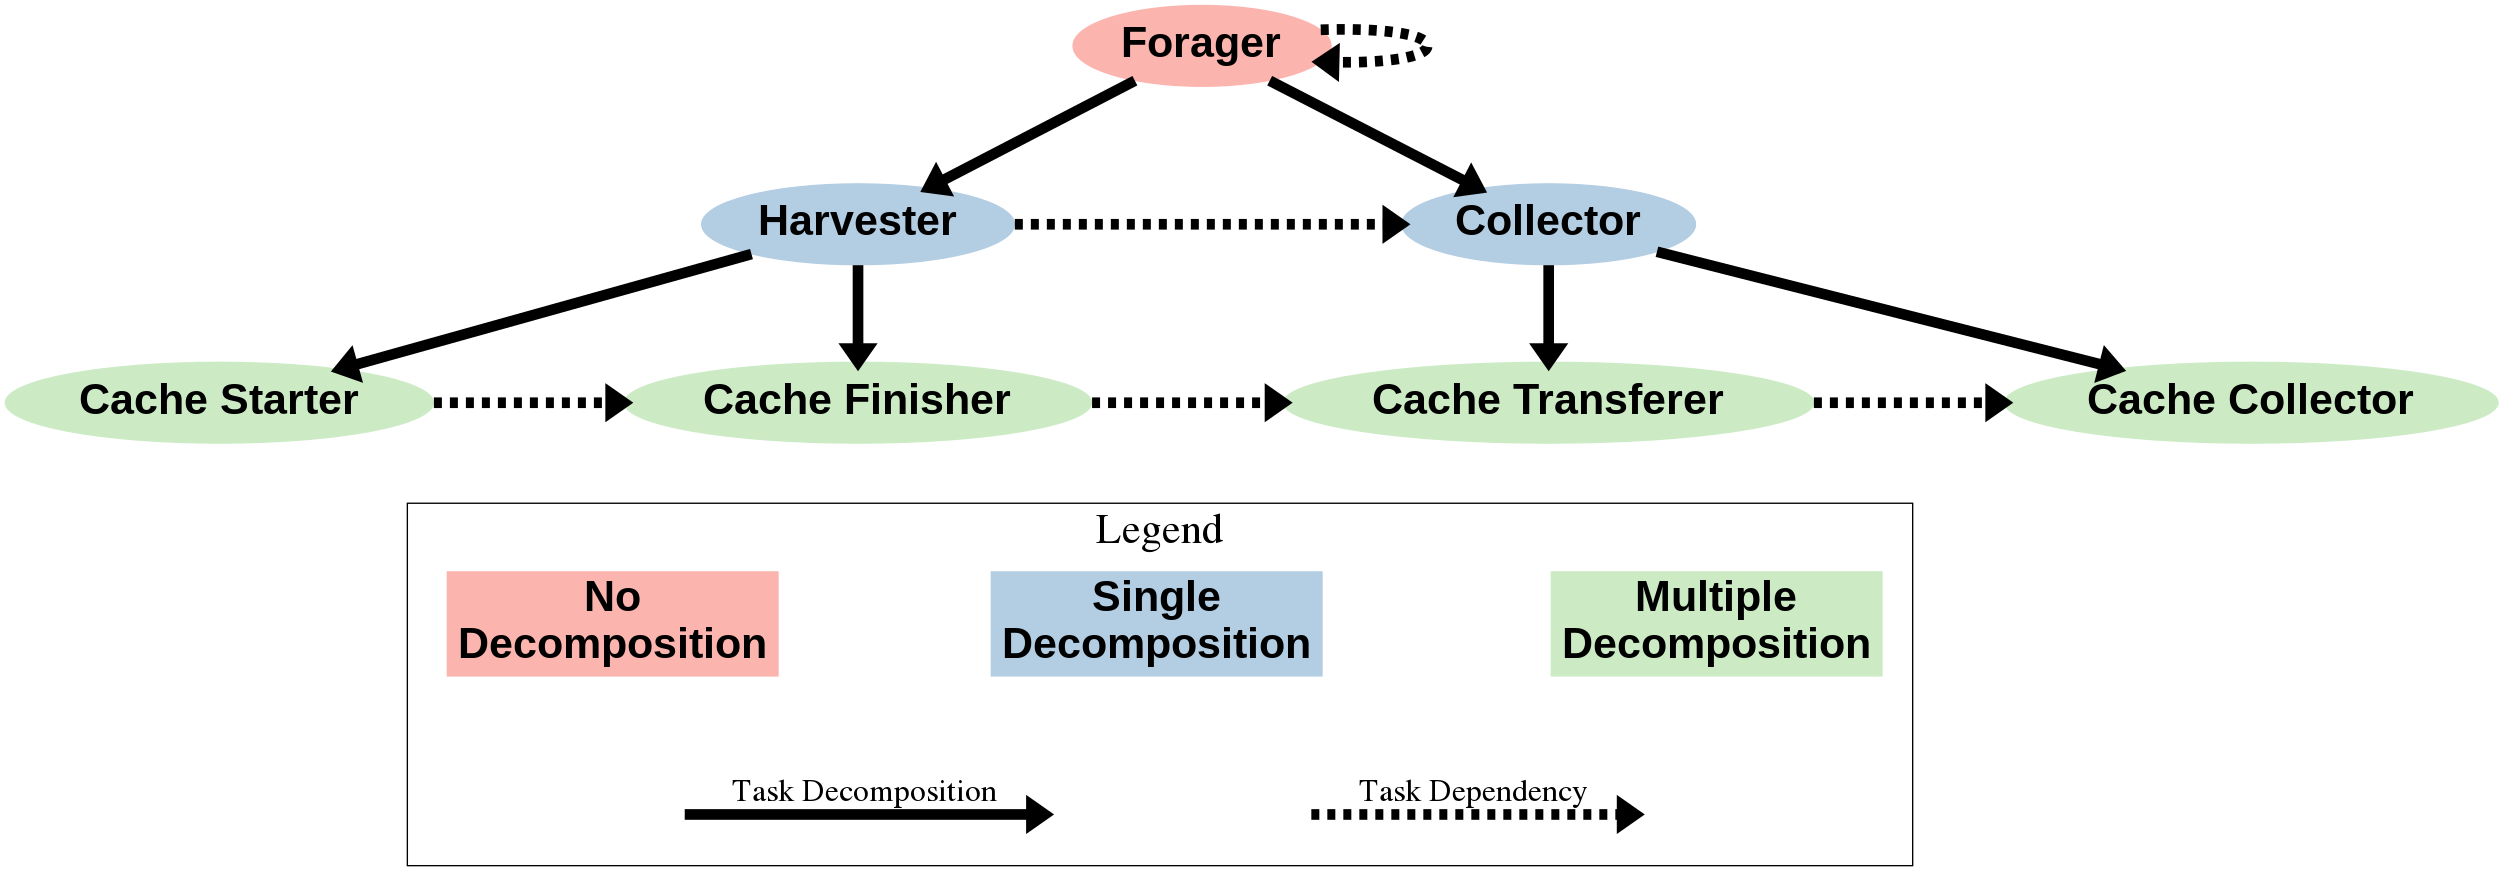
\includegraphics[width=\textwidth]{figures/chapter2/tdgraph-foraging.png}
  \caption[Task decomposition graph, $\TDGraph$, for a foraging
  task, in which robots have to
   find spatially distributed objects in the environment and then bring them to
   a central location.]{\label{fig:tdgraph-foraging}
   Red+blue tasks correspond to a scheme in which robots do
   a whole task or 1/2 task (single decomposition option).  Red+blue+green tasks
   correspond to a scheme in which robots do a whole task, 1/2 task, or 1/4 task
   (multi-decomposition option).  However, by choosing to decompose the task
   into multiple parts, there now exist task dependencies between the parts,
   which the swarm has to collectively learn to be successful.
   Blue tasks ($\phi_i=1$) were defined in~\cite{Harwell2018}, green tasks
   ($\phi_i=2$) were defined~\cite{Harwell2019a}.}
\end{figure}

\begin{itemize}
\item \emph{Forager}: Acquire a free block of highest utility and bring it to the
  nest. This is $\TAGraphRoot$, and one way of accomplishing the swarm objective
  $\SwarmObjective$ via $\phi_0$.

\item \emph{Harvester}: Acquire a free block of highest utility and bring it to the
  existing cache of highest utility, calculated as:
%
  \begin{equation}\label{eqn:existing-cache-utility}
    \mu_{\hat{C_j}}(t) = \frac{e^{-\tau_{\hat{C_j}}(t)}{\lvert \hat{C_j} \rvert}}{\norm{\ArbRobot - \mathbf{C_j}}\norm{\mathbf{C_j} - \mathbf{nest}}}
  \end{equation}
%
  where $\lvert \hat{C_j} \rvert$ is the estimated size of the $j$th cache known to
  $\ArbRobot$ (caches might not exist anymore, and therefore a robot only has
  estimates of their existence). This equation emphasizes selection of caches that
  are close to the position of $\ArbRobot$, but also that are closer to the nest,
  while accounting for the relevancy of a robot's information about
  $C_j$~\cite{Harwell2018}. This task accomplishes part of $\SwarmObjective$ via
  $\phi_1$.

\item \emph{Collector} Acquire a block from the existing cache of highest utility
  (Eqn.~\eqref{eqn:existing-cache-utility}) and bring it to the nest. This task
  accomplishes part of $\SwarmObjective$ via $\phi_1$.
\end{itemize}
%
We extend prior work with the following tasks, implemented as vertices comprising the
task sequence $\phi_2$ (red vertices in Fig.~\ref{fig:tdgraph-foraging}):

\begin{itemize}
\item {\emph{Cache Starter}: Acquire a free block of highest utility and bring it
    partway back to the nest, and then drop it at a feasible site to start a \emph{De
      Novo} cache, according to Eqn.~\eqref{eqn:cache-site-select}. A feasible site
    is one at least a distance $\eta$ from all known caches
    $\hat{C_1}\ldots\hat{C_n}$.
    %
    The best cache site \textbf{x} for $\ArbRobot$ is computed as follows:
    %
    \arraycolsep=0.75pt
    \begin{equation}
      \label{eqn:cache-site-select}
      \begin{array}{lc}
        \underset{\mathbf{x}}{\max} & \mu_{\ArbRobot} \\
        \text{s.t.} & \norm{\mathbf{x} - \mathbf{\hat{C_{m}}}} \geq \eta, \; m = 1, \ldots, n. \\
      \end{array}
    \end{equation}
    where
    \begin{equation}
      \label{eqn:cache-site-utility}
      \mu_{\ArbRobot} = {\Big(\norm{\mathbf{x} -\mathbf{x}_{\ArbRobot}} \norm{\mathbf{x} - \frac{\mathbf{x}_{\ArbRobot} - \mathbf{nest}}{2}}\Big)}^{-1} \\
    \end{equation}

    % [JRH] see if I can find some natural analogues of this sort of utility--would
    % really strengthen my choice of utility function
    Intuitively, cache sites that are close to $\mathbf{x}_{\ArbRobot}$ are better
    (less work to get to, less chance of being found unsuitable upon arrival), as are
    sites that are close to the halfway point between the robot's current position
    and the nest (bisecting the space maximizes available areas for \emph{Collector}
    and \emph{Harvester} tasks, reducing interference). This task accomplishes part
    of $\SwarmObjective$ via $\phi_2$.}

\item {\emph{Cache Finisher}: Acquire a free block of highest utility and place it
    within a distance $\eta$ to a \emph{De Novo} cache (a single free block a
    distance $\eta$ from all other blocks) of maximum utility
    (Eqn.~\eqref{eqn:existing-cache-utility} with $\lvert\hat{C_j}\rvert = 1$) in
    order to create a new cache. This task accomplishes part of $\SwarmObjective$ via
    $\phi_2$.}

\item {\emph{Cache Transferer}: Acquire a block from the existing cache of highest
    utility and transport it to the existing cache with the second highest
    utility. This accomplishes part of $\SwarmObjective$ via $\phi_2$.  }
\item {\emph{Cache Collector}: Acquire a block from the existing cache of highest
    utility (Eqn.~\eqref{eqn:existing-cache-utility}) and bring it to the nest. This
    task accomplishes part of $\SwarmObjective$ via $\phi_2$.}
\end{itemize}

By defining $\phi_2$, we have also implicitly defined $\beta_1,\beta_2$.

\section{Foraging Scenarios}\label{sec:exp-foraging-scenarios}

% [JRH] Show pictures of all the scenarios here, talk a little about each (e.g.,
% why PL is the most challenging scenario type).

\section{Source Code}\label{sec:exp-source-code}

% [JRH] Put a few bits about SIERRA/TITERRA in here.

Our open-source code is available at https://github.com/swarm-robotics/fordyca,
https://github.com/swarm-robotics/silicon,
https://github.com/swarm-robotics/sierra, and
https://github.com/swarm-robotics/titerra.

%%% Local Variables:
%%% mode: latex
%%% TeX-master: "../thesis"
%%% End:


%%%%%%%%%%%%%%%%%%%%%%%%%%%%%%%%%%%%%%%%%%%%%%%%%%%%%%%%%%%%%%%%%%%%%%%%%%%%%%%%
% app-glossary.tex: Glossary Appendix:
%%%%%%%%%%%%%%%%%%%%%%%%%%%%%%%%%%%%%%%%%%%%%%%%%%%%%%%%%%%%%%%%%%%%%%%%%%%%%%%%
\chapter{Glossary and Acronyms}%
\label{app:glossary}
%%%%%%%%%%%%%%%%%%%%%%%%%%%%%%%%%%%%%%%%%%%%%%%%%%%%%%%%%%%%%%%%%%%%%%%%%%%%%%%%
Care has been taken in this thesis to minimize the use of jargon and
acronyms, but this cannot always be achieved.  This appendix defines
jargon terms in a glossary, and contains a table of acronyms and their
meaning.
%%%%%%%%%%%%%%%%%%%%%%%%%%%%%%%%%%%%%%%%%%%%%%%%%%%%%%%%%%%%%%%%%%%%%%%%%%%%%%%%

%%%%%%%%%%%%%%%%%%%%%%%%%%%%%%%%%%%%%%%%%%%%%%%%%%%%%%%%%%%%%%%%%%%%%%%%%%%%%%%%
% Glossary
%%%%%%%%%%%%%%%%%%%%%%%%%%%%%%%%%%%%%%%%%%%%%%%%%%%%%%%%%%%%%%%%%%%%%%%%%%%%%%%%
\printglossary

%%%%%%%%%%%%%%%%%%%%%%%%%%%%%%%%%%%%%%%%%%%%%%%%%%%%%%%%%%%%%%%%%%%%%%%%%%%%%%%%
% Acronyms
%%%%%%%%%%%%%%%%%%%%%%%%%%%%%%%%%%%%%%%%%%%%%%%%%%%%%%%%%%%%%%%%%%%%%%%%%%%%%%%%
\printglossary[type=\acronymtype]

%%% Local Variables:
%%% mode: latex
%%% TeX-master: "../thesis"
%%% End:


%%%%%%%%%%%%%%%%%%%%%%%%%%%%%%%%%%%%%%%%%%%%%%%%%%%%%%%%%%%%%%%%%%%%%%%%%%%%%%%%
% THE THESIS ENDS
%%%%%%%%%%%%%%%%%%%%%%%%%%%%%%%%%%%%%%%%%%%%%%%%%%%%%%%%%%%%%%%%%%%%%%%%%%%%%%%%
\end{document}


%%% Local Variables:
%%% mode: latex
%%% TeX-master: t
%%% End:
